---
id: moments-likes-three-years
title: 朋友圈点赞的三年
date: 2026-11-02
authors: x1shang
venue: 描述性分析 · 化名版
summary: 基于近三年 20 条动态、860 次点赞与 161 位独立点赞者，考察点赞的时间分布、内容差异和核心受众，并以全历史数据作补充分析。
abstract: 内容、时机与核心受众：基于本机微信数据的描述性分析。数据截止 2026-11-02，文中人名均为化名。
tags: [朋友圈, 点赞, 时间动力学, 内容类型, 社会网络, 描述性统计]
---
% 站点副本：正文、统计、图表及附录来自用户提供的化名版 TeX。
% 仅做网页排版适配：文档头移至元信息；图宏展开为 figure；图表编号与交叉引用显式化；
% PNG 使用站内资源路径；移除印刷分页、重复表头与目录指令。原始包逐字节保存在 source.zip。
\noindent 数据截止 2026-11-02。文中人名均为化名。

\href{assets/papers/moments-likes-analysis/source.zip}{下载 TeX 源码与化名数据（ZIP）}

\section*{摘要}
目的：考察近三年朋友圈点赞的时间分布、内容类型差异与核心点赞者。方法：以本机微信数据库为数据源，选取 2023-11-01 至 2026-10-31 的 20 条本人动态，提取 860 次他人点赞、110 条他人评论和 161 位独立点赞者；采用描述统计、20,000 次 bootstrap 区间、Spearman 相关与 Kruskal--Wallis 检验；另以 46 条全历史动态作趋势拟合与阶段补充，不用于主结论。结果：46.6\% 的赞在 1 小时内、74.5\% 在 6 小时内、92.6\% 在 24 小时内到达，中位半衰期为 1.15 小时；长文/月报平均 58.5 赞，城市/影像 48.7，旅行/自然 42.0，校园/成长 40.7，技术/项目 35.8，类别差异不显著（$p=0.431$）；前四位点赞者各 18/20，前 10\% 点赞者贡献 31.3\%，Gini 系数为 0.466。结论：点赞集中在发布后一天内；内容类型差异仅具描述意义；核心点赞圈规模小且稳定；发布时间影响点赞速度，而非最终总量。全历史补充分析显示，八年点赞数呈显著线性上升（$\beta=5.40$ 赞/年，95\% CI 4.29--6.52，$R^2=0.671$），学校阶段队列与两次大考前后呈现不同的参与结构。

\noindent{\textbf{关键词：}朋友圈；点赞；时间动力学；内容类型；社会网络；描述性统计}

\section{1 数据与方法}

\subsection{1.1 数据来源与样本}
数据来自本机微信 4.1.15.56 的 SQLCipher 数据库 \texttt{sns.db}，读取时间为 2026-11-02。数据库中共有 47 条发布者为本账号的动态；其中 1 条为 2023-12-31 16:46 的重复空帖（1 图、无正文、无互动），剔除后余 46 条。另有 4 次自赞被剔除。

主分析限定最近 36 个月（2023-11-01 至 2026-10-31），共 20 条动态，获得 860 次他人点赞、110 条他人评论（不含本人回复）和 161 位独立点赞者。其余 26 条早期动态仅用于第 3 节的趋势拟合与阶段补充。联系人是否仍在好友列表不影响纳入；已删除联系人的历史点赞仍保留在样本中。

\subsection{1.2 变量与指标}
点赞数按 wxid 去重，自赞不计；评论数为他人评论，不含本人回复。点赞延迟定义为点赞时间减去发布时间；半衰期定义为累计赞数首次达到该帖最终赞数 50\% 的时间；首小时占比定义为发布后 1 小时内的赞数占最终赞数的比例。

主样本按正文主题分为五类：长文/月报、城市/影像、技术/项目、旅行/自然、校园/成长。编码为人工单编码，优先依据正文主题；图文并茂时以文字主题为准。学校阶段（小学、初中、高中、大学）仅用于第 3 节的补充分析，由群聊成员关系推断：群名含相应阶段关键词者归入该阶段；一人可属于多个阶段，补充分析中的“关系”取最早阶段。

\subsection{1.3 统计方法}
均值区间使用 20,000 次 percentile bootstrap；连续关联使用 Spearman 秩相关；类别差异使用 Kruskal--Wallis 检验。全历史趋势使用最小二乘线性回归（点赞数对小数年份），报告斜率、95\% 置信区间与 $R^2$。所有检验为双侧，未做多重比较校正；样本量小，$p$ 值仅作辅助，结论为描述性，不作因果推断。

\section{2 结果}

\subsection{2.1 总量与轨迹}
近三年 20 条动态共获得 860 次他人点赞，均值 \textbf{43.0}，中位 \textbf{41.0}，范围 \textbf{18--69}。年度均值分别为：2023 年 2 条 47.0，2024 年 6 条 34.7，2025 年 6 条 43.7，2026 年 6 条 49.3。2024 年出现回落，2025--2026 年回升；三年样本并不支持“逐年单调上升”的判断。

单条峰值是 2026-04-16 的 18 岁生日帖 \textbf{69 赞}（28 条评论）；其次是 2025-06-13 的《长白山》\textbf{63 赞}；2026-09-11 的《骑行外滩》和 2026-10-31 的《十月月报》各 \textbf{61 赞}。最低为 2026-10-11 的建站帖 \textbf{18 赞}。

\begin{table}[H]
\centering
\caption{表 1：近三年主样本的年度点赞与评论。评论不含本人回复。}
\footnotesize
\begin{tabular}{@{}l r r r r r@{}}
\toprule
年份 & 条数 & 总赞 & 均值 & 中位 & 评论 \\
\midrule
2023 & 2 & 94 & 47.0 & 47.0 & 12 \\
2024 & 6 & 208 & 34.7 & 34.0 & 13 \\
2025 & 6 & 262 & 43.7 & 45.0 & 19 \\
2026 & 6 & 296 & 49.3 & 54.5 & 66 \\
\bottomrule
\end{tabular}
\end{table}

\begin{figure}
\centering
\href{assets/papers/moments-likes-analysis/fig1_main_timeline.png}{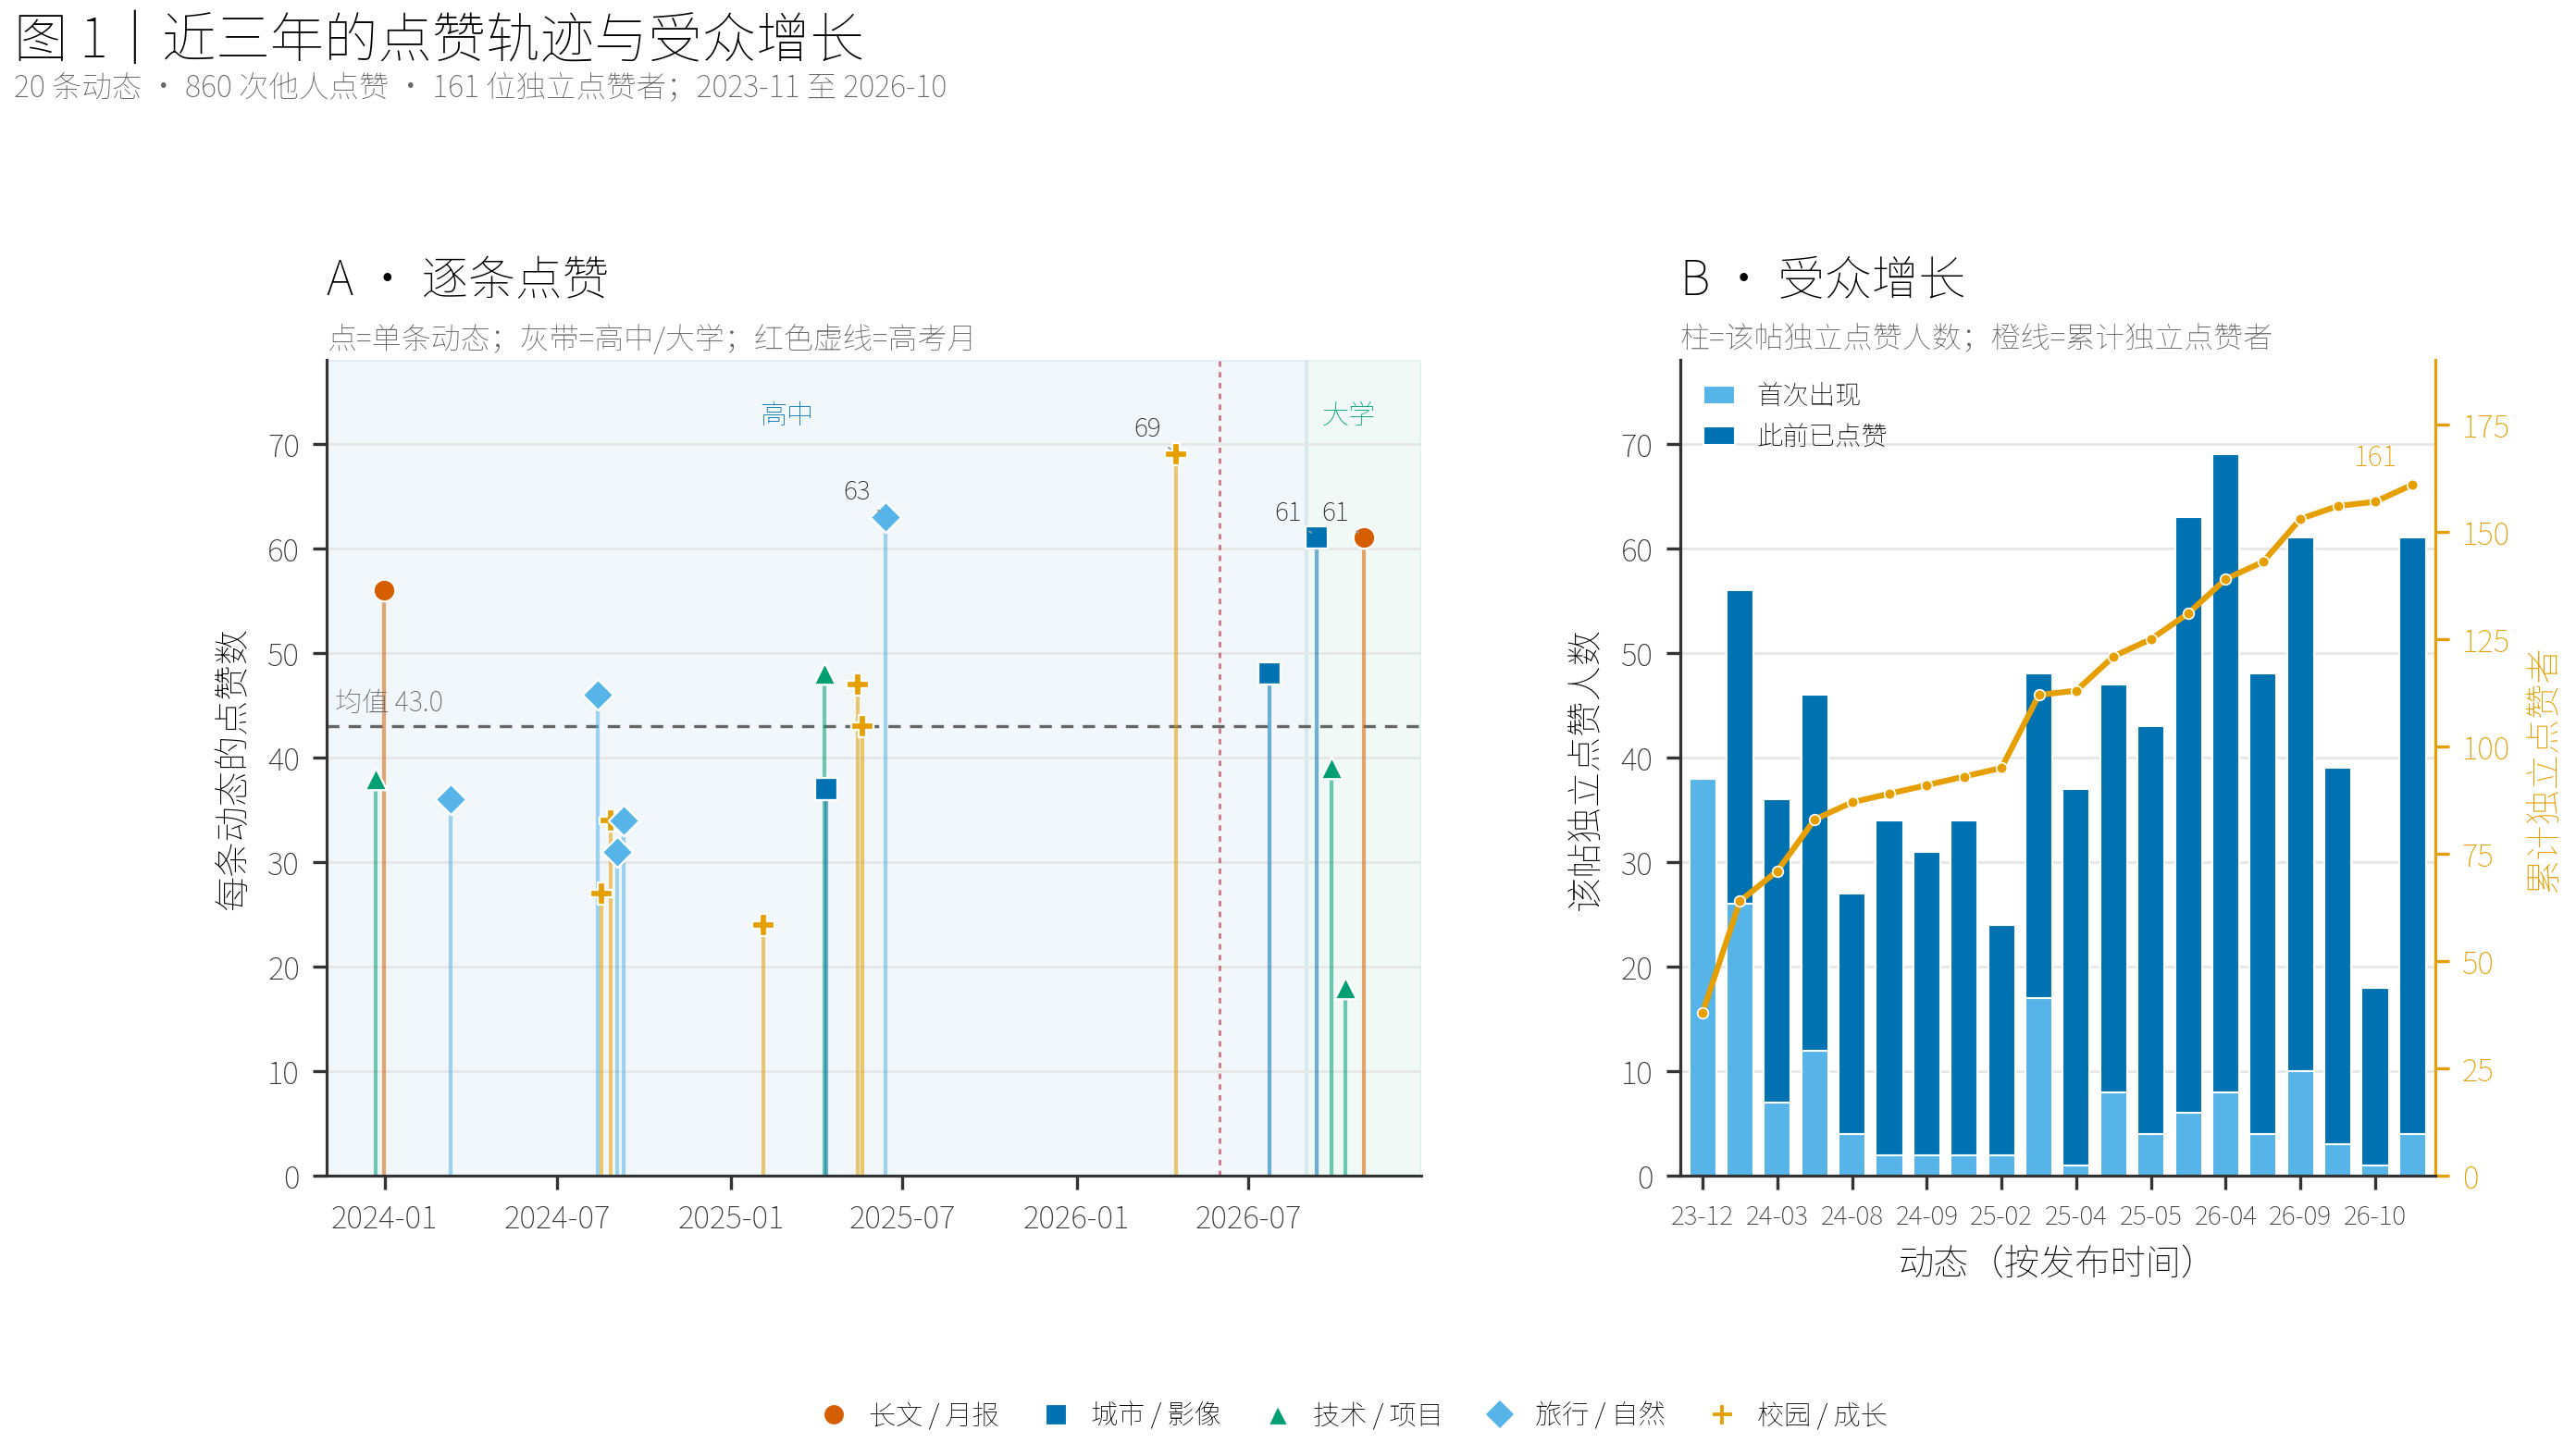
\includegraphics{assets/papers/moments-likes-analysis/fig1_main_timeline.png}}
\caption{图 1：近三年的点赞轨迹与受众增长。A：20 条动态的逐条点赞；灰带=高中/大学；红色虚线=高考月。B：每帖独立点赞者中的新/老面孔与累计独立点赞者。}
\end{figure}

\subsection{2.2 时间动力学}
860 次点赞中，46.6\% 在发布后 1 小时内到达，74.5\% 在 6 小时内，92.6\% 在 24 小时内，96.7\% 在 72 小时内。点赞延迟中位数为 \textbf{1.22 小时}，半衰期中位数为 \textbf{1.15 小时}。一条动态的点赞主要在发布后一天内完成。

发布小时与半衰期呈负相关：越晚发布，半衰期越短（$\rho=-0.67$，$p=0.001$）。但总赞与发布小时几乎无关（$\rho=0.13$，$p=0.58$）。由此可见，发布时间主要改变点赞到达的速度，而不是最终规模。

\begin{figure}
\centering
\href{assets/papers/moments-likes-analysis/fig2_main_temporal.png}{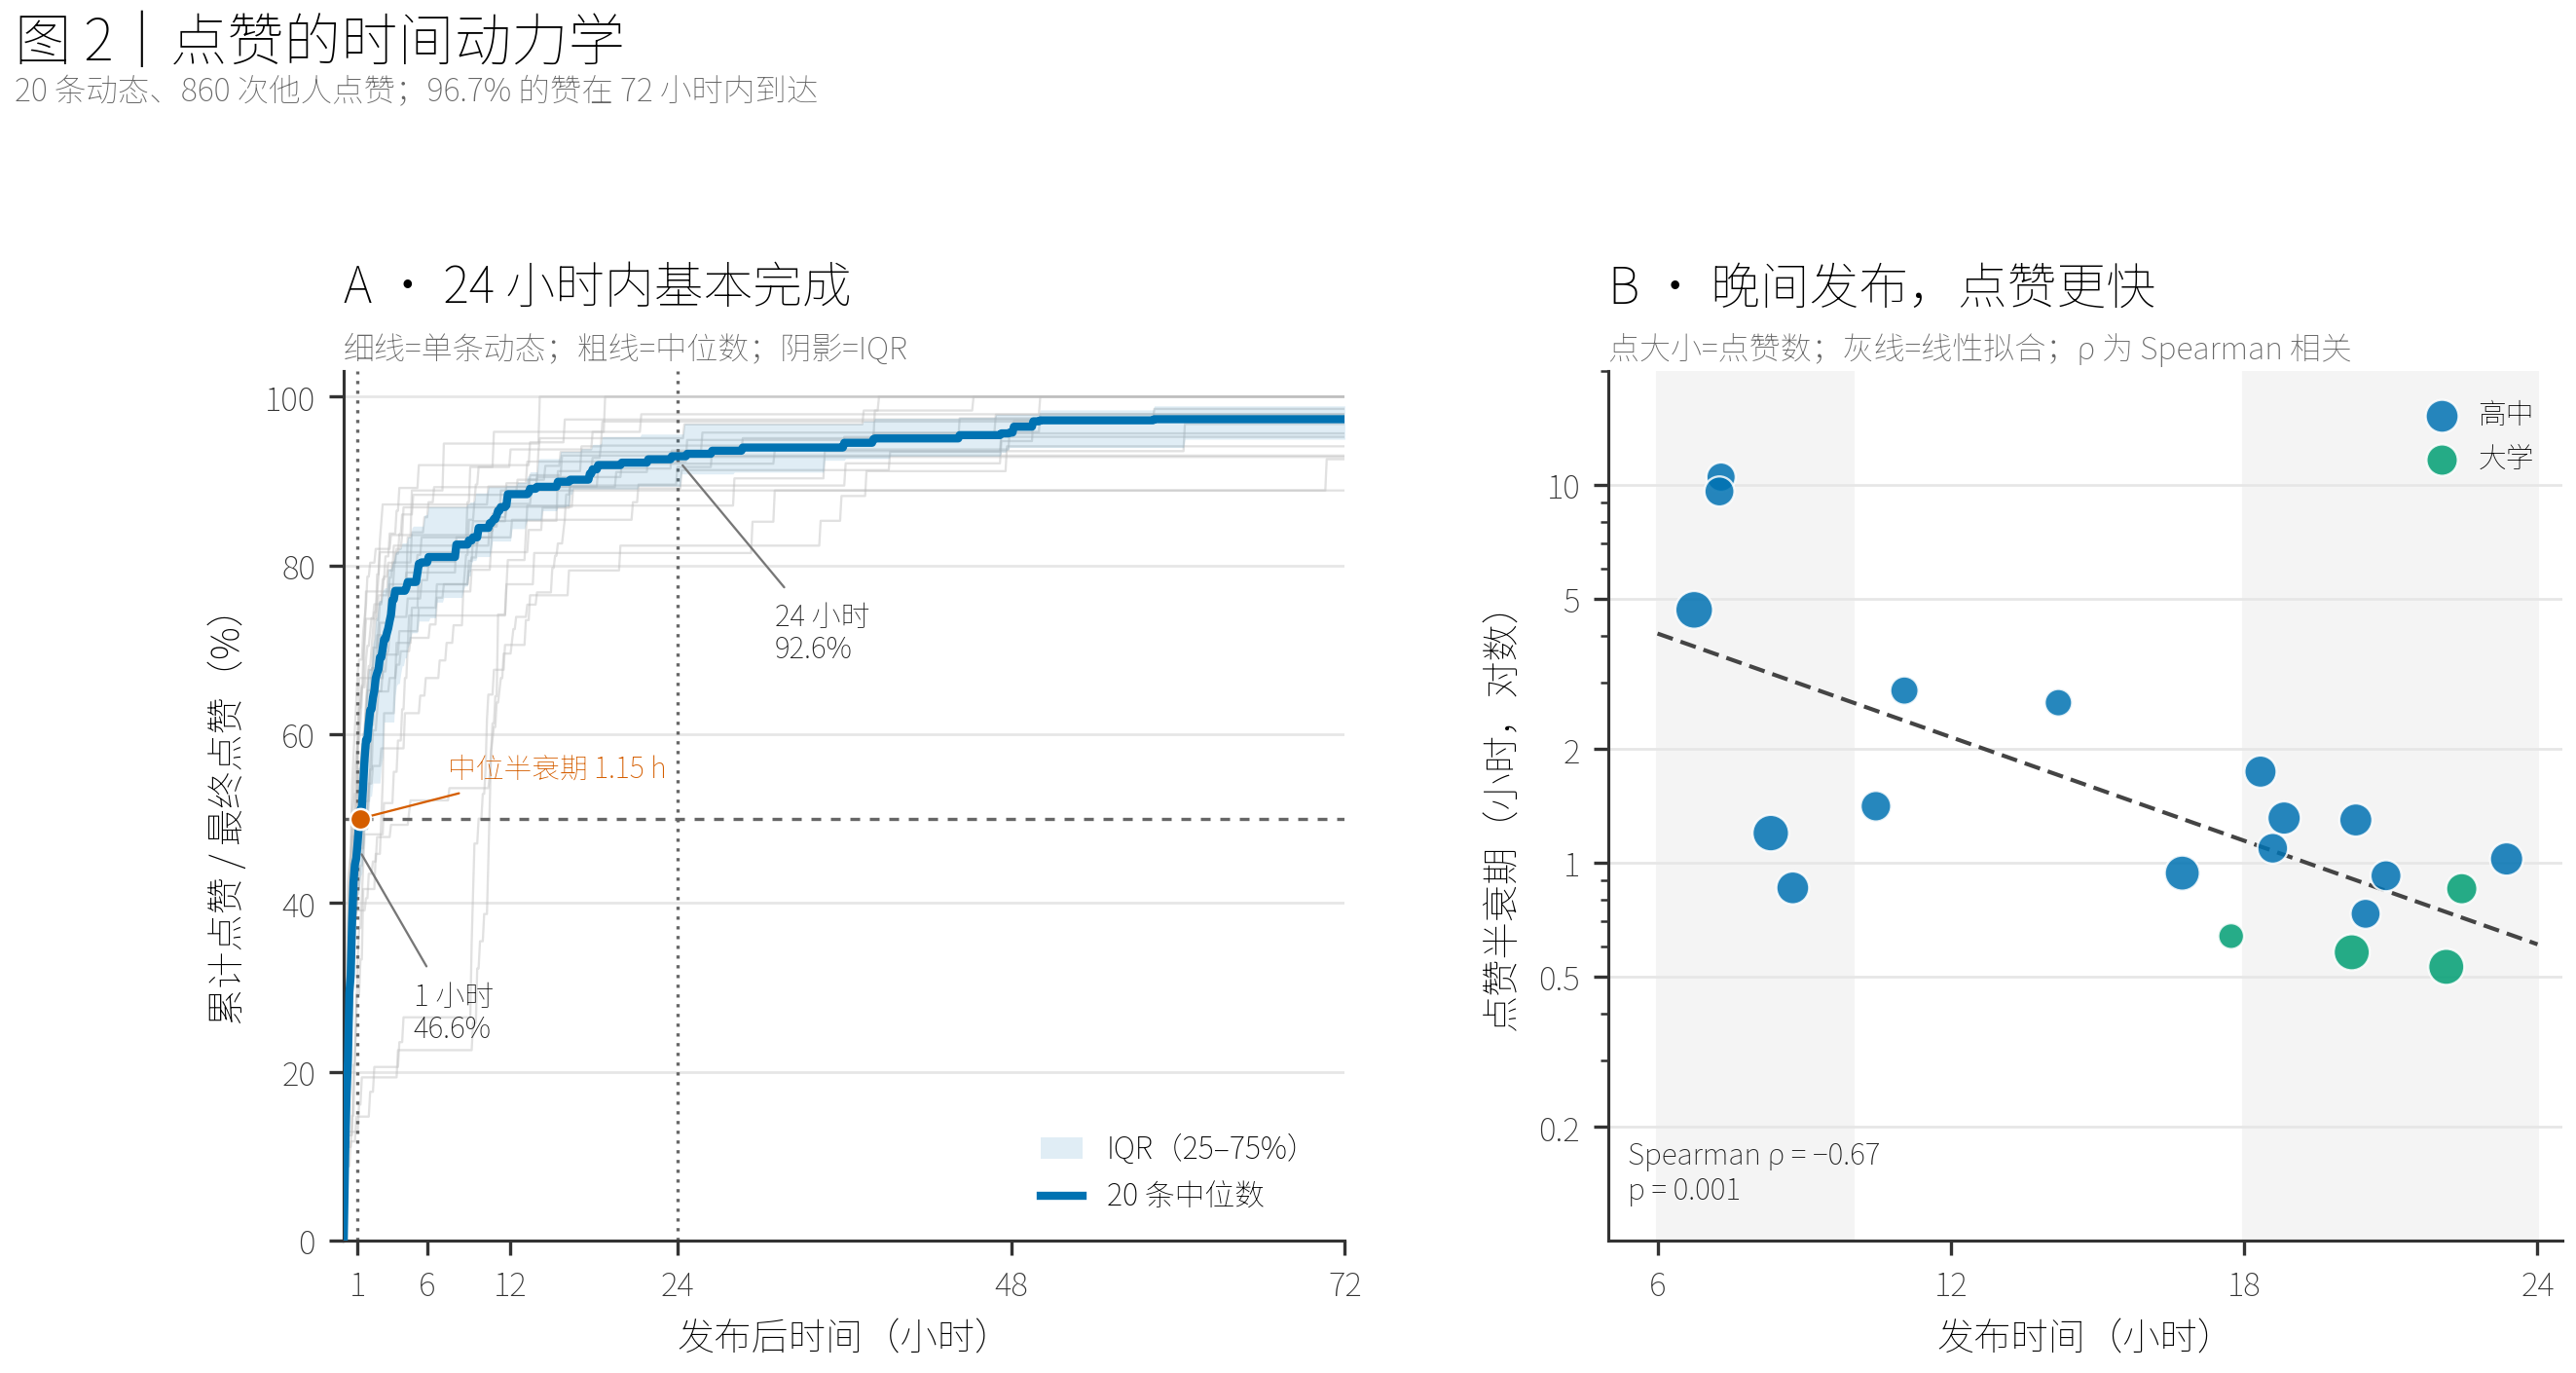
\includegraphics{assets/papers/moments-likes-analysis/fig2_main_temporal.png}}
\caption{图 2：点赞的时间动力学。A：20 条动态的点赞累积曲线（中位数与 IQR）；B：发布时间与半衰期，颜色=学校阶段，点大小=点赞数。}
\end{figure}

\subsection{2.3 内容类型}
五类动态的均值分别为：长文/月报 \textbf{58.5}（$n=2$）、城市/影像 \textbf{48.7}（$n=3$）、旅行/自然 \textbf{42.0}（$n=5$）、校园/成长 \textbf{40.7}（$n=6$）、技术/项目 \textbf{35.8}（$n=4$）。Kruskal--Wallis 检验 $p=0.431$，类别差异不显著；上述排序仅作描述，不能据此推断内容类型的普遍效应。

评论维度与点赞并不一致。技术/项目的评论/赞比为 19\%，校园/成长 18\%，长文/月报 12\%，城市/影像 11\%，旅行/自然 4\%。技术/项目与校园/成长更偏“讨论型”，长文/月报更偏“认可型”，旅行/自然更偏“欣赏型”。

\begin{table}[H]
\centering
\caption{表 2：近三年五类内容的点赞与评论。评论/赞为组内汇总。}
\footnotesize
\begin{tabular}{@{}l r r r r r@{}}
\toprule
类型 & n & 均值 & 中位 & 评论均值 & 评论/赞 \\
\midrule
长文 / 月报 & 2 & 58.5 & 58.5 & 7.0 & 12\% \\
城市 / 影像 & 3 & 48.7 & 48.0 & 5.3 & 11\% \\
旅行 / 自然 & 5 & 42.0 & 36.0 & 1.8 & 4\% \\
校园 / 成长 & 6 & 40.7 & 38.5 & 7.3 & 18\% \\
技术 / 项目 & 4 & 35.8 & 38.5 & 6.8 & 19\% \\
\bottomrule
\end{tabular}
\end{table}

\begin{figure}
\centering
\href{assets/papers/moments-likes-analysis/fig3_main_categories.png}{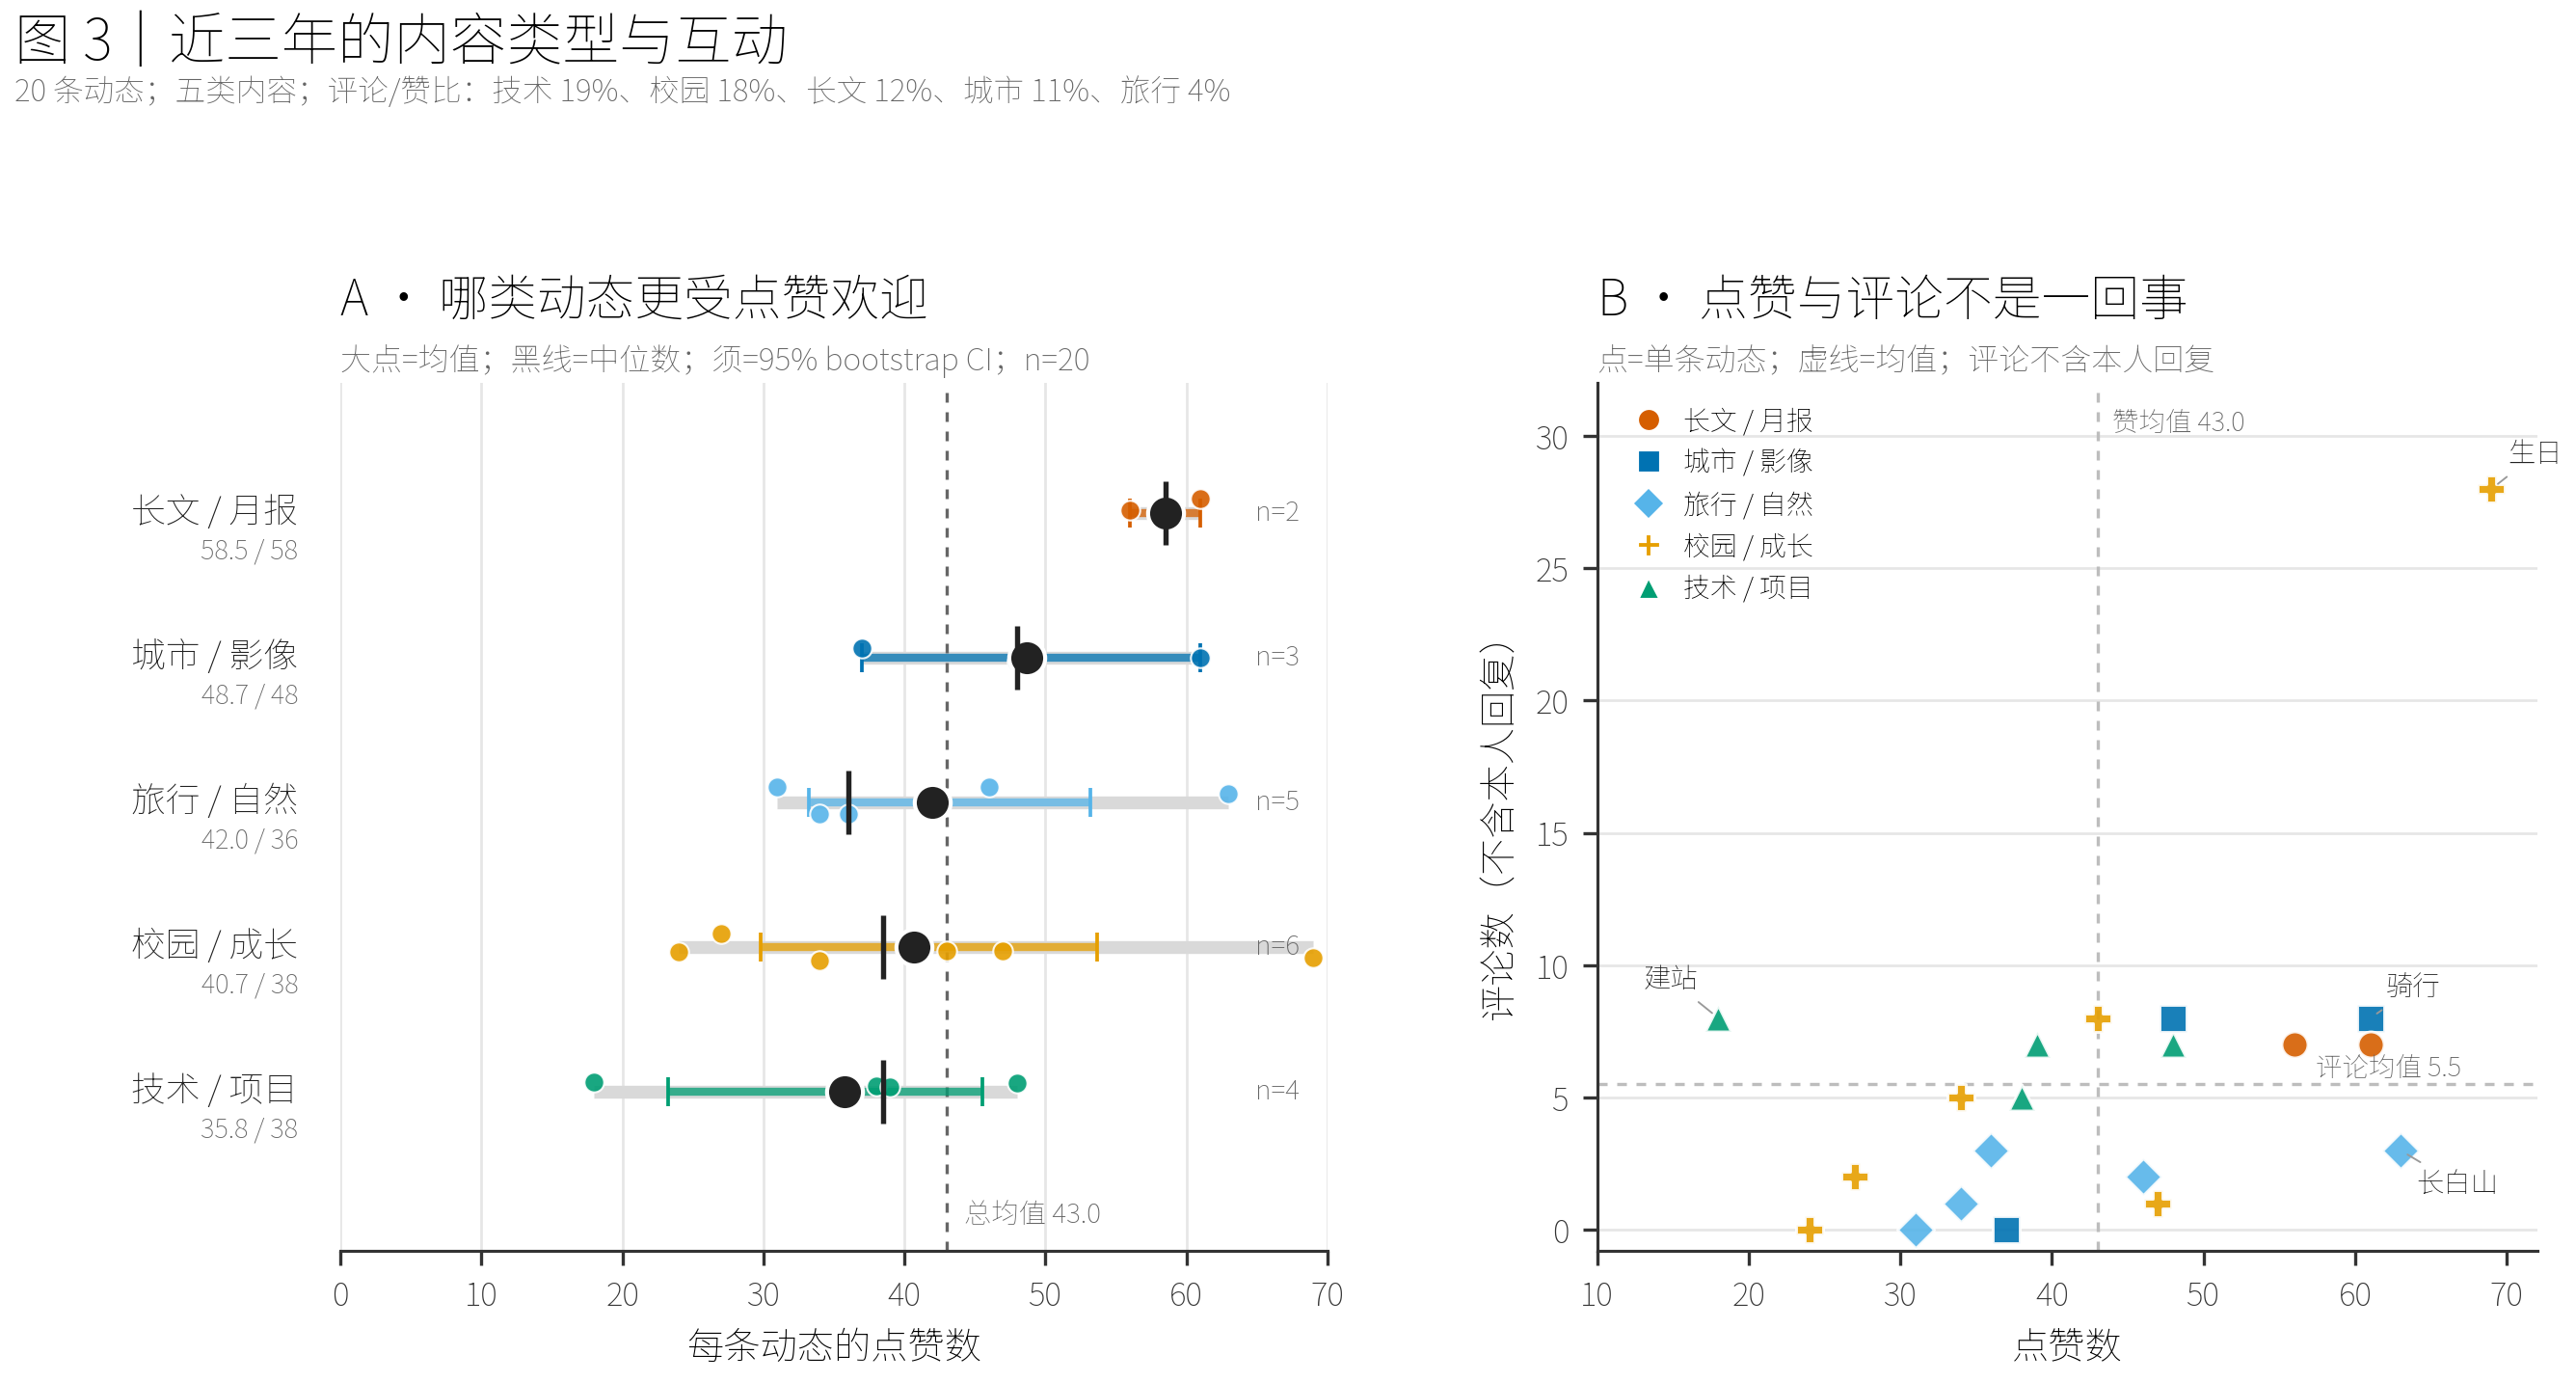
\includegraphics{assets/papers/moments-likes-analysis/fig3_main_categories.png}}
\caption{图 3：近三年的内容类型与互动。A：五类动态的点赞分布（均值、中位数与 95\% bootstrap CI）；B：点赞与评论的关系。}
\end{figure}

\subsection{2.4 核心点赞者}
161 位点赞者共贡献 860 次赞。前四位各点赞 18/20 条动态（90\%），随后四位各 17/20 条（85\%）；前 10 人贡献 20.0\% 的赞。点赞次数最多的 15 位见表~3。

“经常”不等于“迅速”。前 15 位的中位点赞延迟从约 0.3 小时到 7 小时不等；高频点赞者内部存在明显的速度差异。表~3 同时给出延迟中位数。

\begin{table}[H]
\centering
\caption{表 3：近三年点赞次数最多的 15 位。延迟中位为小时。}
\footnotesize
\begin{tabular}{@{}r p{2.2cm} r r p{2.1cm}@{}}
\toprule
\# & 姓名 & 点赞数 & /20 & 延迟中位（h） \\
\midrule
1 & ZZD & 18 & 90\% & 0.56 \\
2 & ZAK & 18 & 90\% & 1.34 \\
3 & XAZ & 18 & 90\% & 0.66 \\
4 & MNZ & 18 & 90\% & 0.62 \\
5 & TYS & 17 & 85\% & 0.41 \\
6 & MUZ & 17 & 85\% & 1.40 \\
7 & XLY & 17 & 85\% & 1.20 \\
8 & HIZ & 17 & 85\% & 0.91 \\
9 & TIX & 16 & 80\% & 0.29 \\
10 & XYZ & 16 & 80\% & 2.04 \\
11 & HZ & 15 & 75\% & 0.92 \\
12 & ZSI & 14 & 70\% & 1.22 \\
13 & MDY & 14 & 70\% & 7.20 \\
14 & XQZ & 14 & 70\% & 0.32 \\
15 & UGL & 14 & 70\% & 0.53 \\
\bottomrule
\end{tabular}
\end{table}

\begin{figure}
\centering
\href{assets/papers/moments-likes-analysis/fig4_main_likers_anon.png}{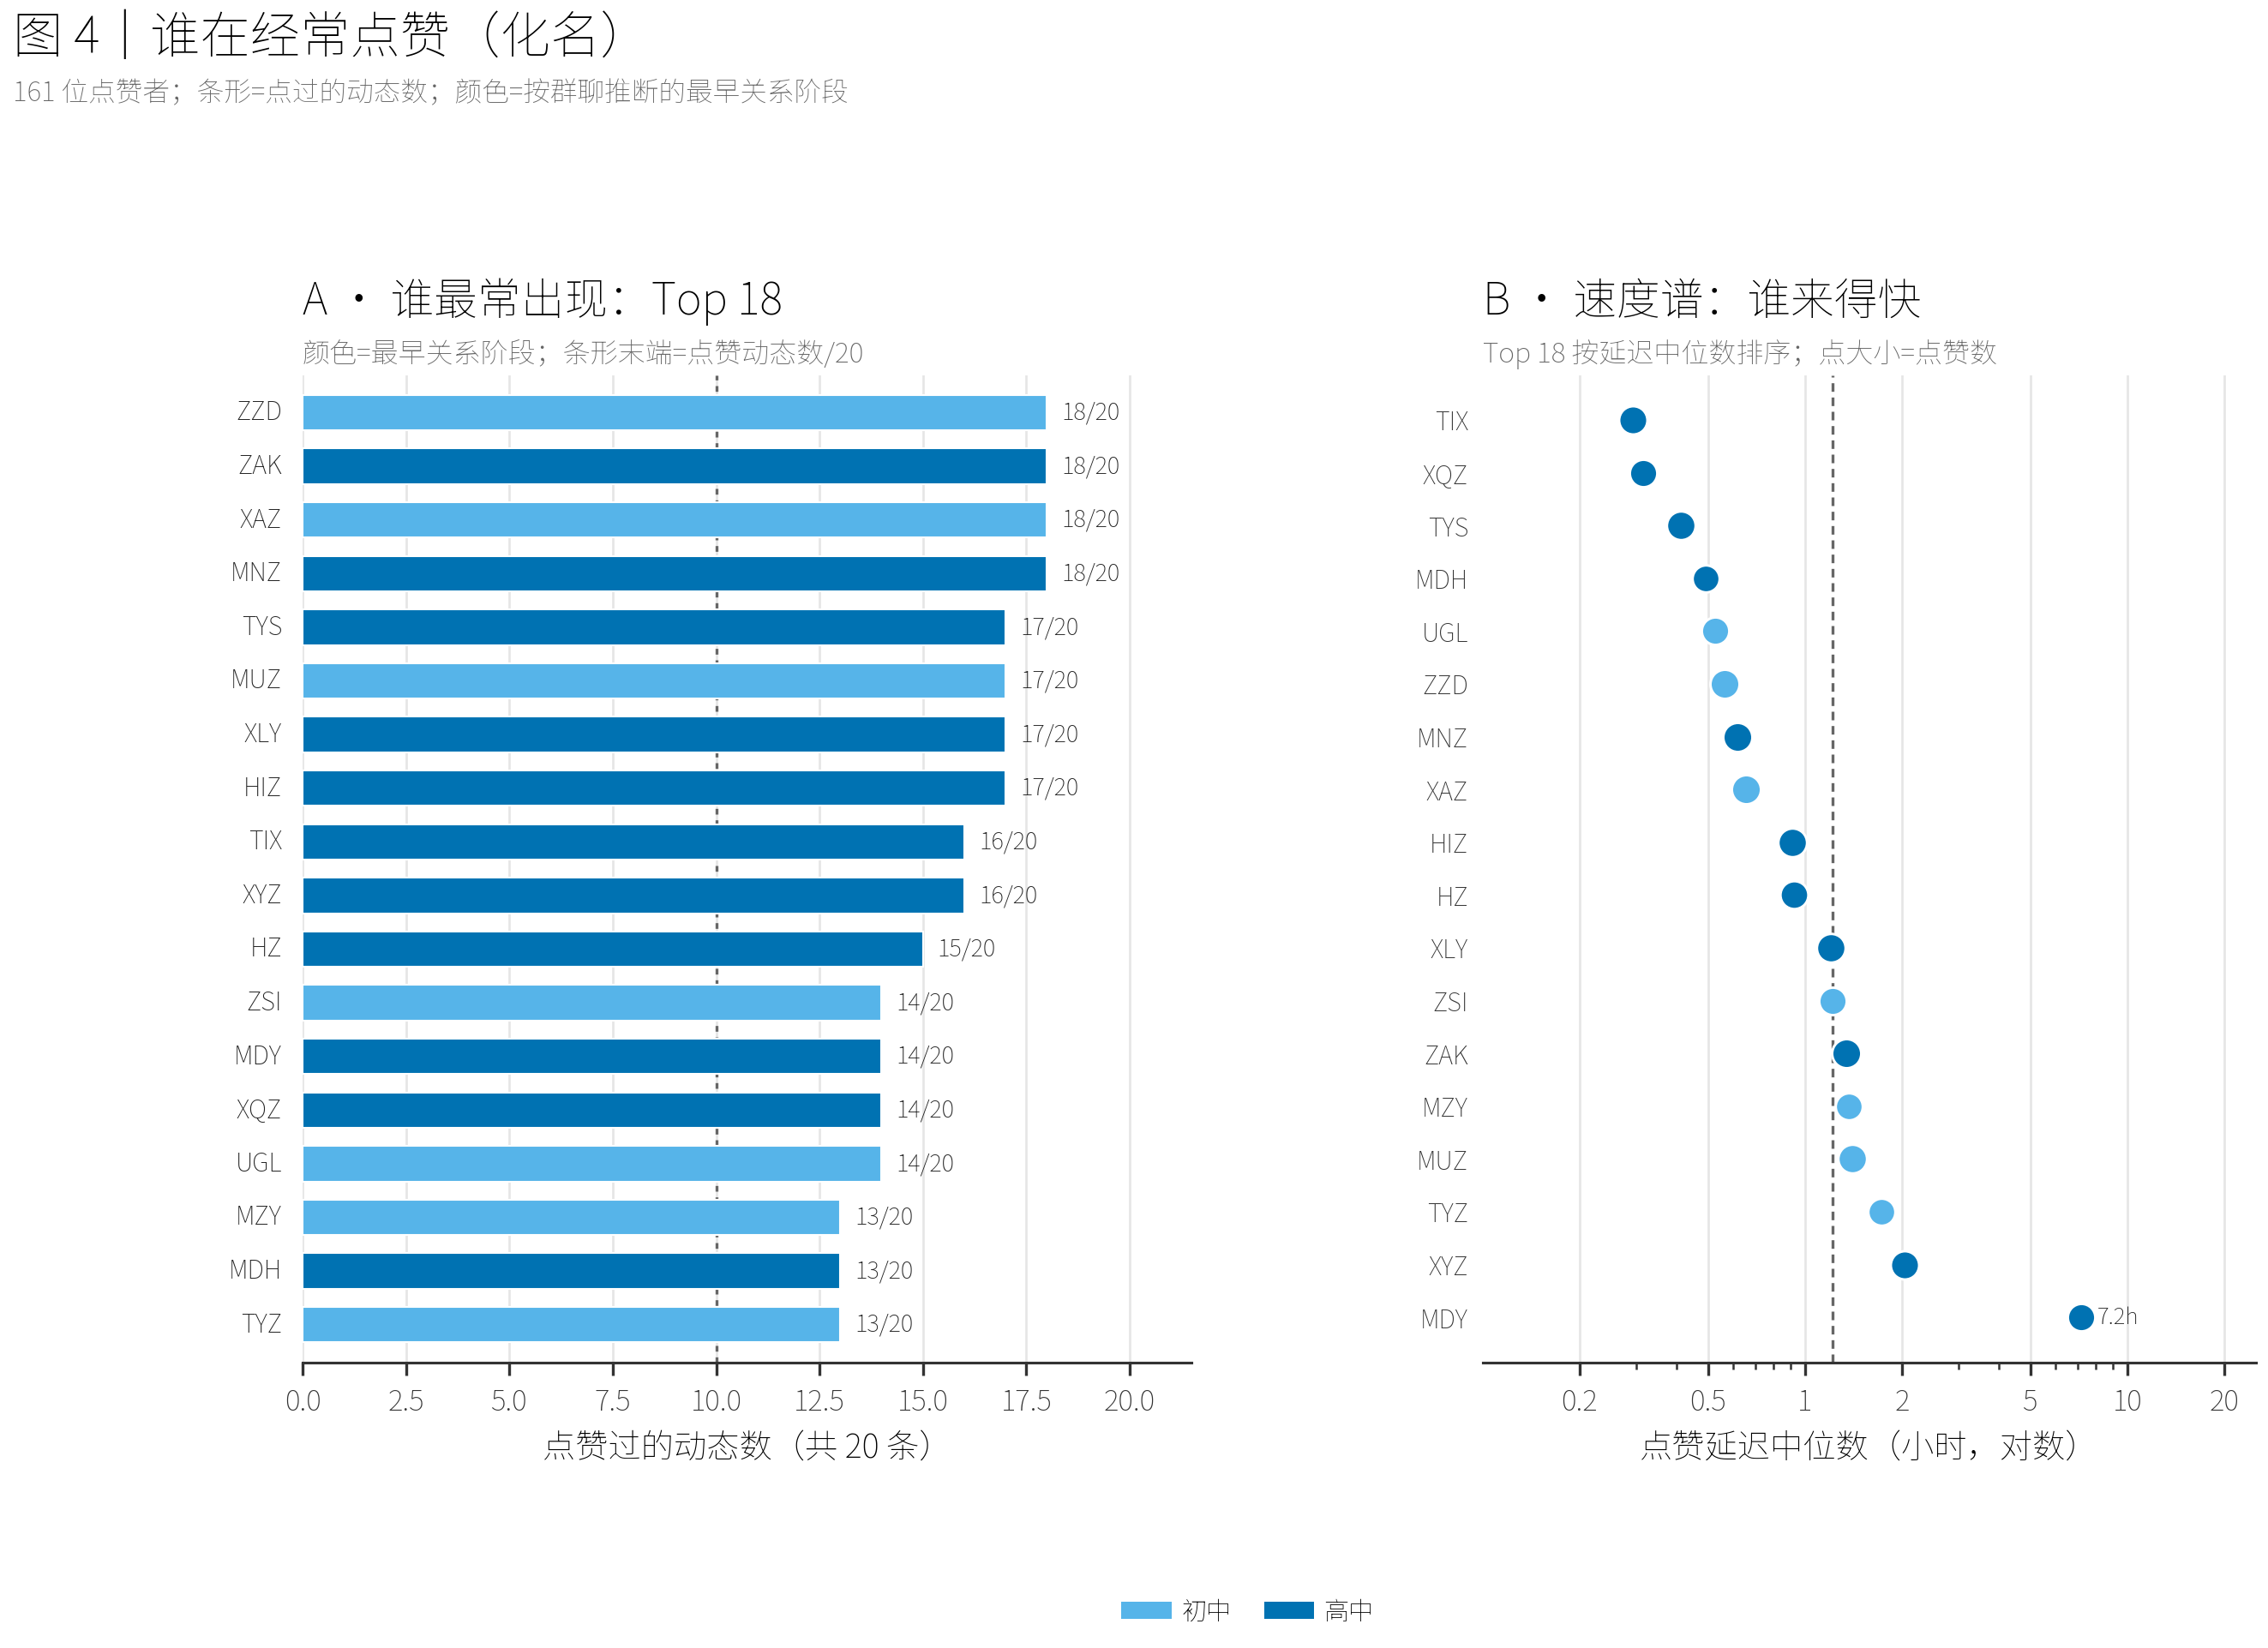
\includegraphics{assets/papers/moments-likes-analysis/fig4_main_likers_anon.png}}
\caption{图 4：近三年核心点赞者。A：点赞次数最多的 18 位；B：其点赞延迟中位数；颜色=最早关系阶段。}
\end{figure}

\subsection{2.5 集中度}
点赞分布呈“稳定核心 + 大长尾”结构。前 10\% 点赞者（17 人）贡献 31.3\%，前 20\%（33 人）贡献 51.2\%，Gini 系数为 \textbf{0.466}。核心并非少数人垄断，但前 8 位的点赞覆盖率达到 85\%--90\%，明显高于长尾。图~5 为相应的洛伦兹曲线。

\begin{figure}
\centering
\href{assets/papers/moments-likes-analysis/fig5_main_lorenz.png}{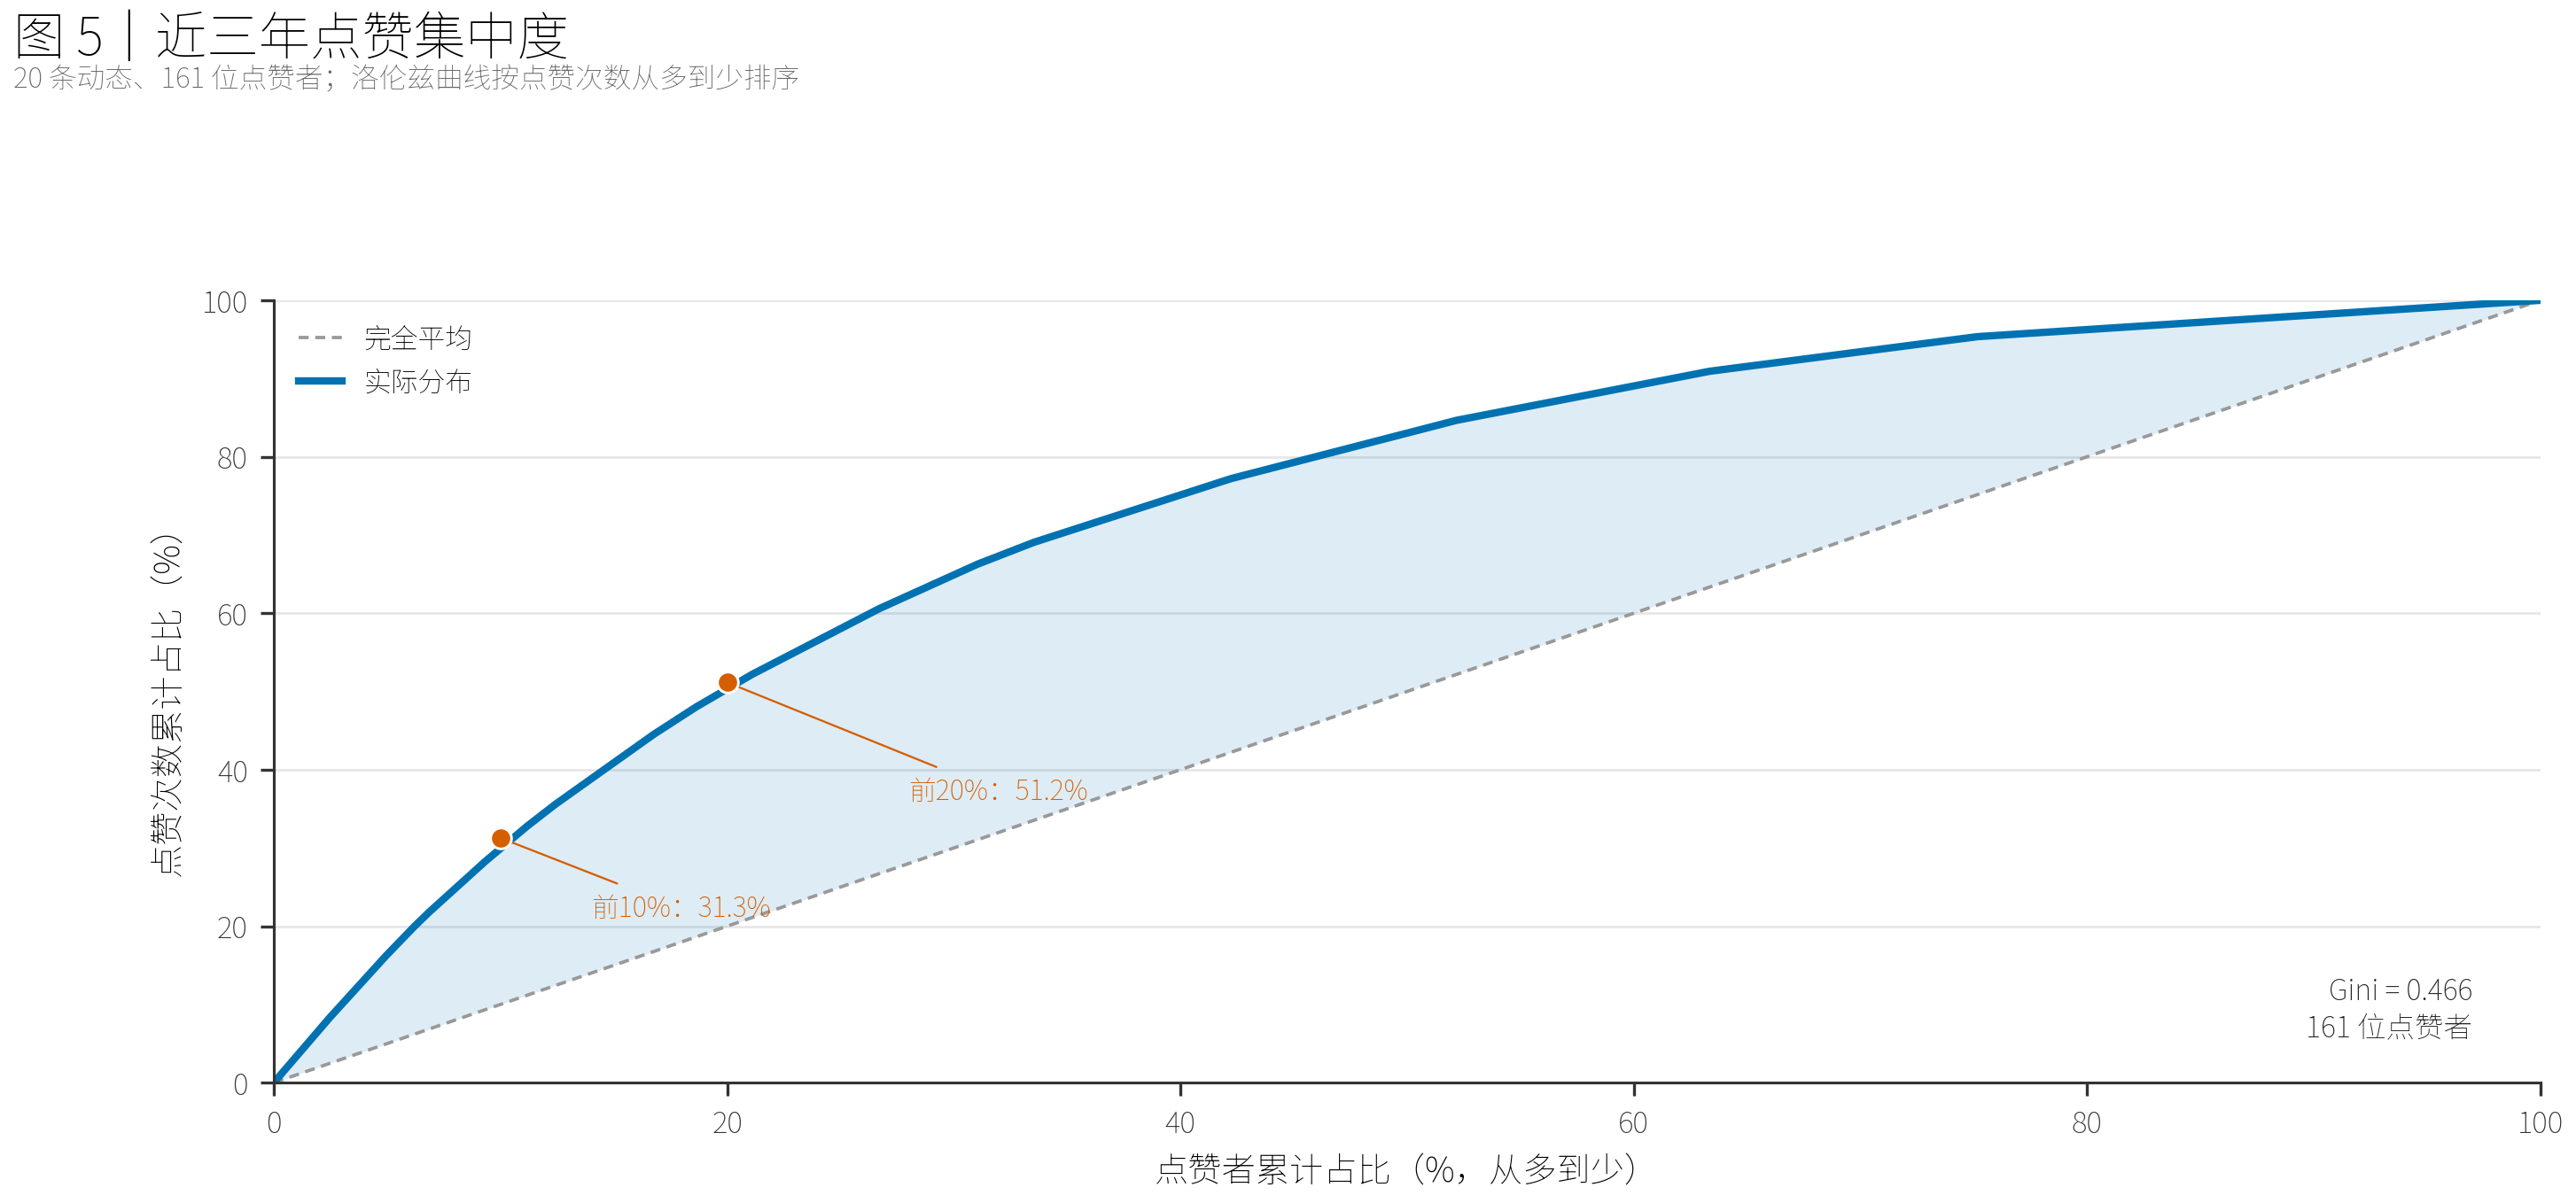
\includegraphics{assets/papers/moments-likes-analysis/fig5_main_lorenz.png}}
\caption{图 5：近三年点赞集中度。洛伦兹曲线按点赞次数从多到少排序；虚线=完全平均。}
\end{figure}

\section{3 补充分析：全历史趋势、阶段与两次大考}

本节使用全部 46 条动态，仅提供纵向背景，不改变第 2 节基于近 36 个月的结论。点赞数随年份系统增长，故以线性拟合描述趋势，并报告斜率、置信区间与拟合优度。

\subsection{3.1 长期趋势}
46 条动态的点赞数随年份显著上升：线性拟合斜率为 \textbf{+5.40 赞/年}（95\% CI 4.29--6.52），$R^2=0.671$，$p<0.001$。这一趋势与受众规模、年龄和平台使用习惯的变化一致，不能直接解释为内容质量的提升。

\begin{figure}
\centering
\href{assets/papers/moments-likes-analysis/figS1_trend.png}{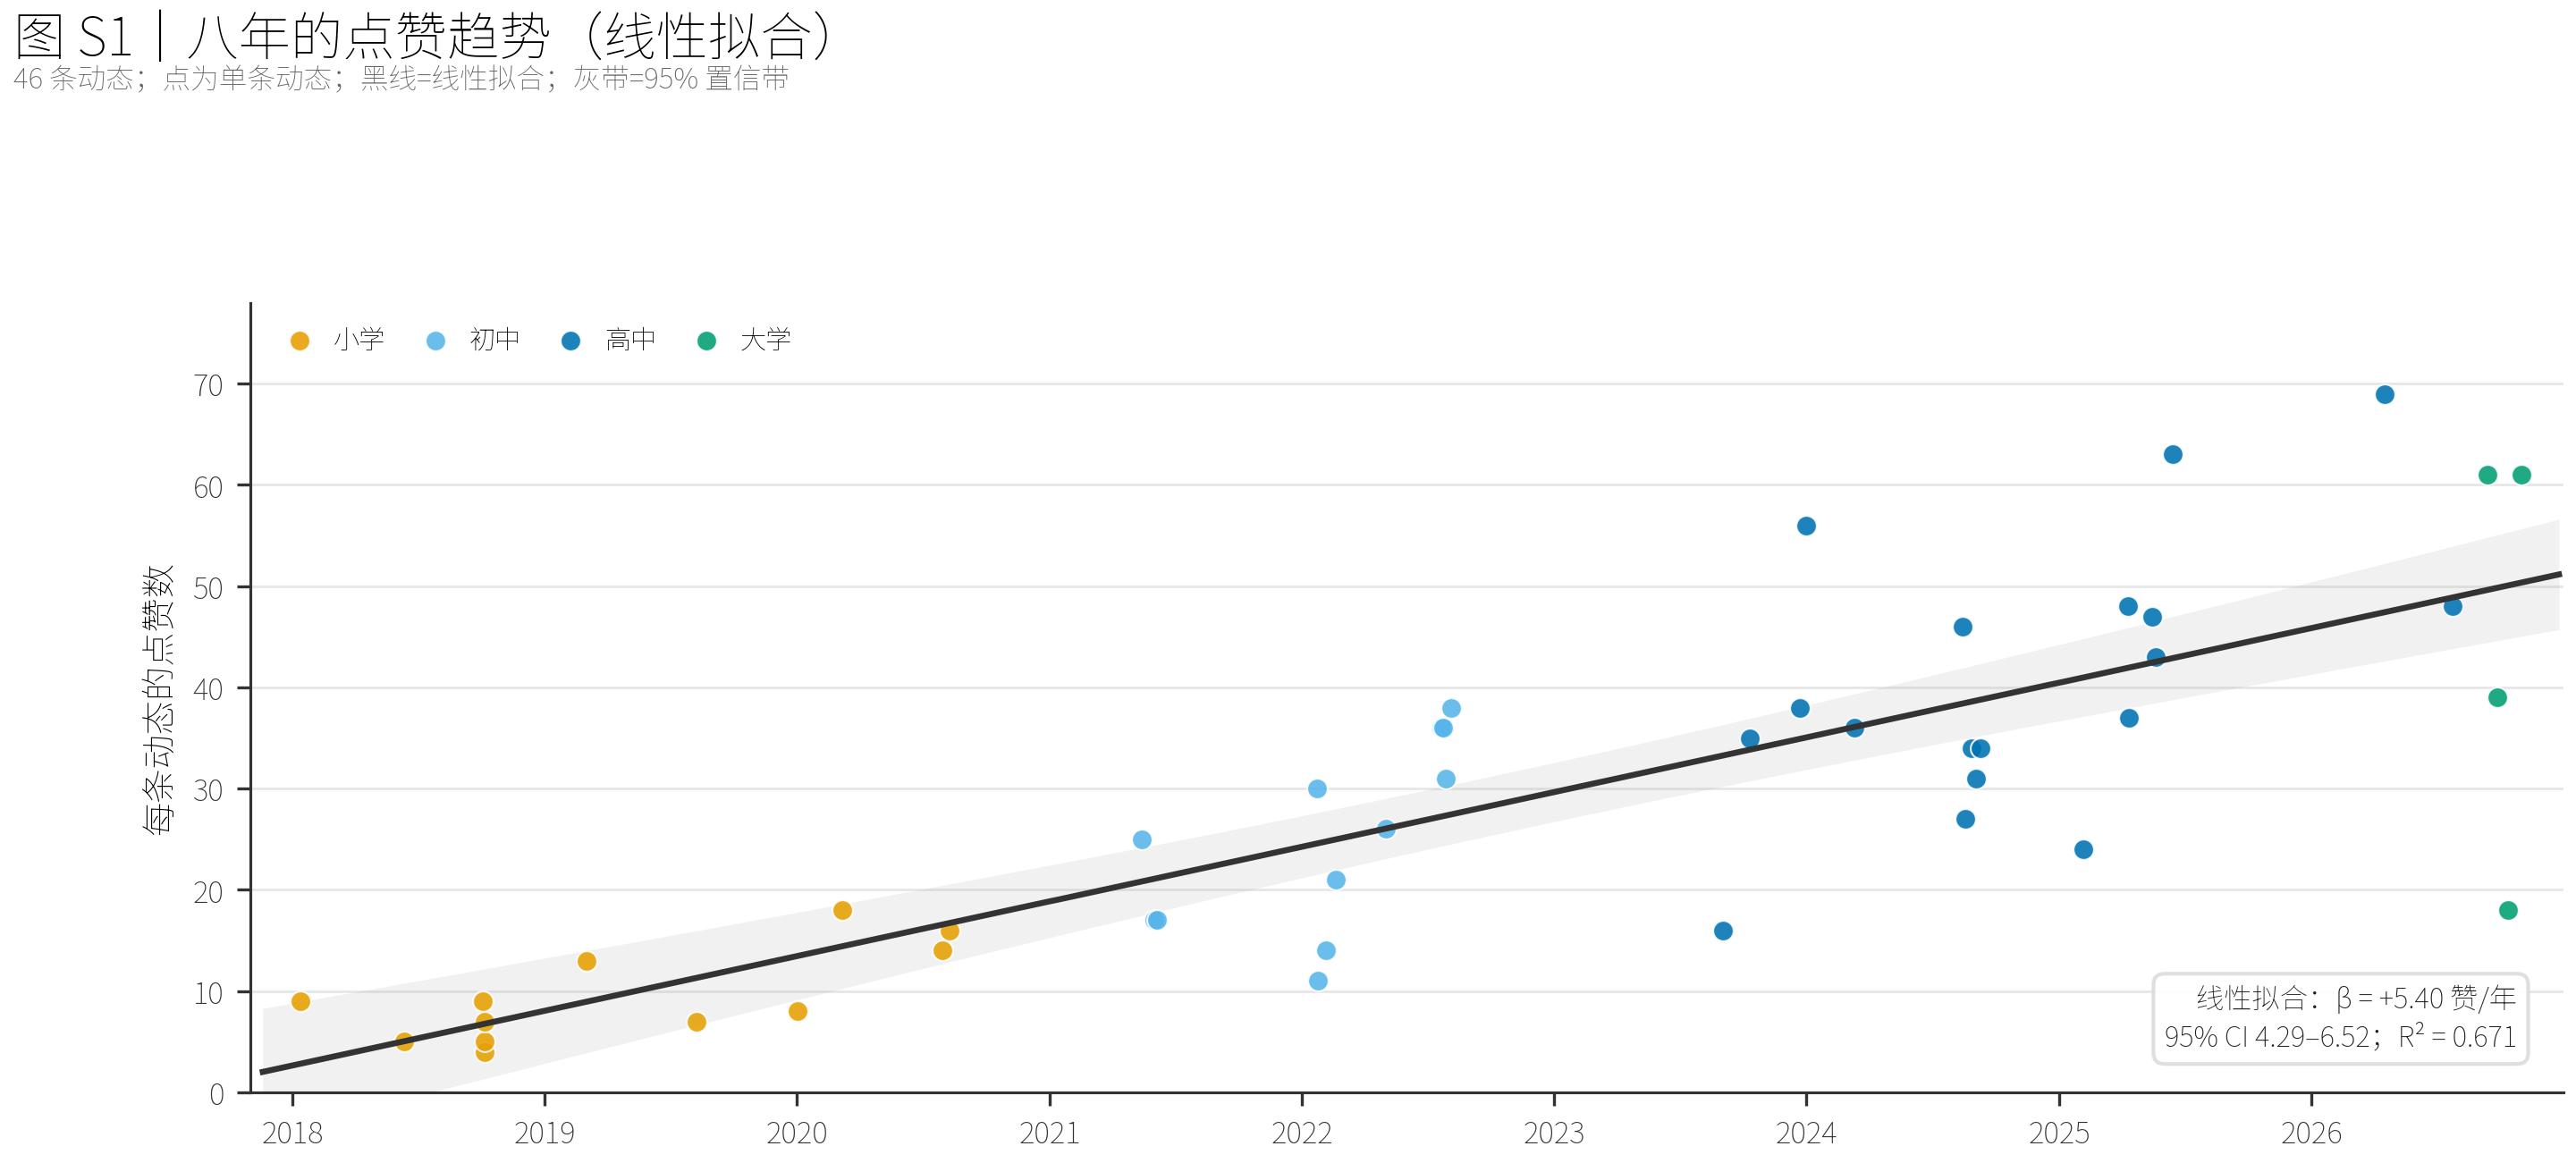
\includegraphics{assets/papers/moments-likes-analysis/figS1_trend.png}}
\caption{图 S1：八年点赞趋势的线性拟合。点为单条动态；黑线=线性拟合；灰带=95\% 置信带。}
\end{figure}

\subsection{3.2 首赞、末赞与学校阶段}
按最早关系阶段分组，小学 32 人，184 次赞（13.9\%），2026 年仍活跃 22\%；初中 38 人，445 次（33.5\%），活跃 63\%；高中 64 人，449 次（33.8\%），活跃 78\%；大学 9 人，21 次（1.6\%），活跃 100\%；其他/未知 49 人，229 次（17.2\%），活跃 55\%。小学与初中合计 629 次，占全部点赞的 \textbf{47.4\%}。

首赞/末赞的阶段构成呈现清晰的队列特征：小学好友 78\% 的首赞发生在小学，末赞分散到小学 28\%、初中 19\%、高中 31\%、大学 22\%；初中好友 79\% 首赞在初中，末赞 50\% 在高中、42\% 在大学；高中好友 97\% 首赞在高中，末赞 42\% 在高中、58\% 在大学；大学好友 100\% 首末均在大学。小学是起点，初中是持续时间最长的桥梁，高中与大学是当前的主要来源。

\begin{table}[H]
\centering
\caption{表 4：全历史点赞者按最早关系阶段的描述统计。2026 活跃=最后一次点赞在 2026 年。}
\footnotesize
\begin{tabular}{@{}l r r r r r l l@{}}
\toprule
阶段 & n & 总赞 & 人均 & 中位 & 2026 活跃 & 首赞中位 & 末赞中位 \\
\midrule
小学 & 32 & 184 & 5.8 & 3.5 & 22\% & 2019-05-21 & 2024-02-04 \\
初中 & 38 & 445 & 11.7 & 9.0 & 63\% & 2022-02-06 & 2026-04-16 \\
高中 & 64 & 449 & 7.0 & 5.0 & 78\% & 2023-12-31 & 2026-09-12 \\
大学 & 9 & 21 & 2.3 & 2.0 & 100\% & 2026-09-11 & 2026-10-11 \\
其他/未知 & 49 & 229 & 4.7 & 4.0 & 55\% & 2022-01-26 & 2026-04-16 \\
\bottomrule
\end{tabular}
\end{table}

\begin{figure}
\centering
\href{assets/papers/moments-likes-analysis/figS2_lifelines_anon.png}{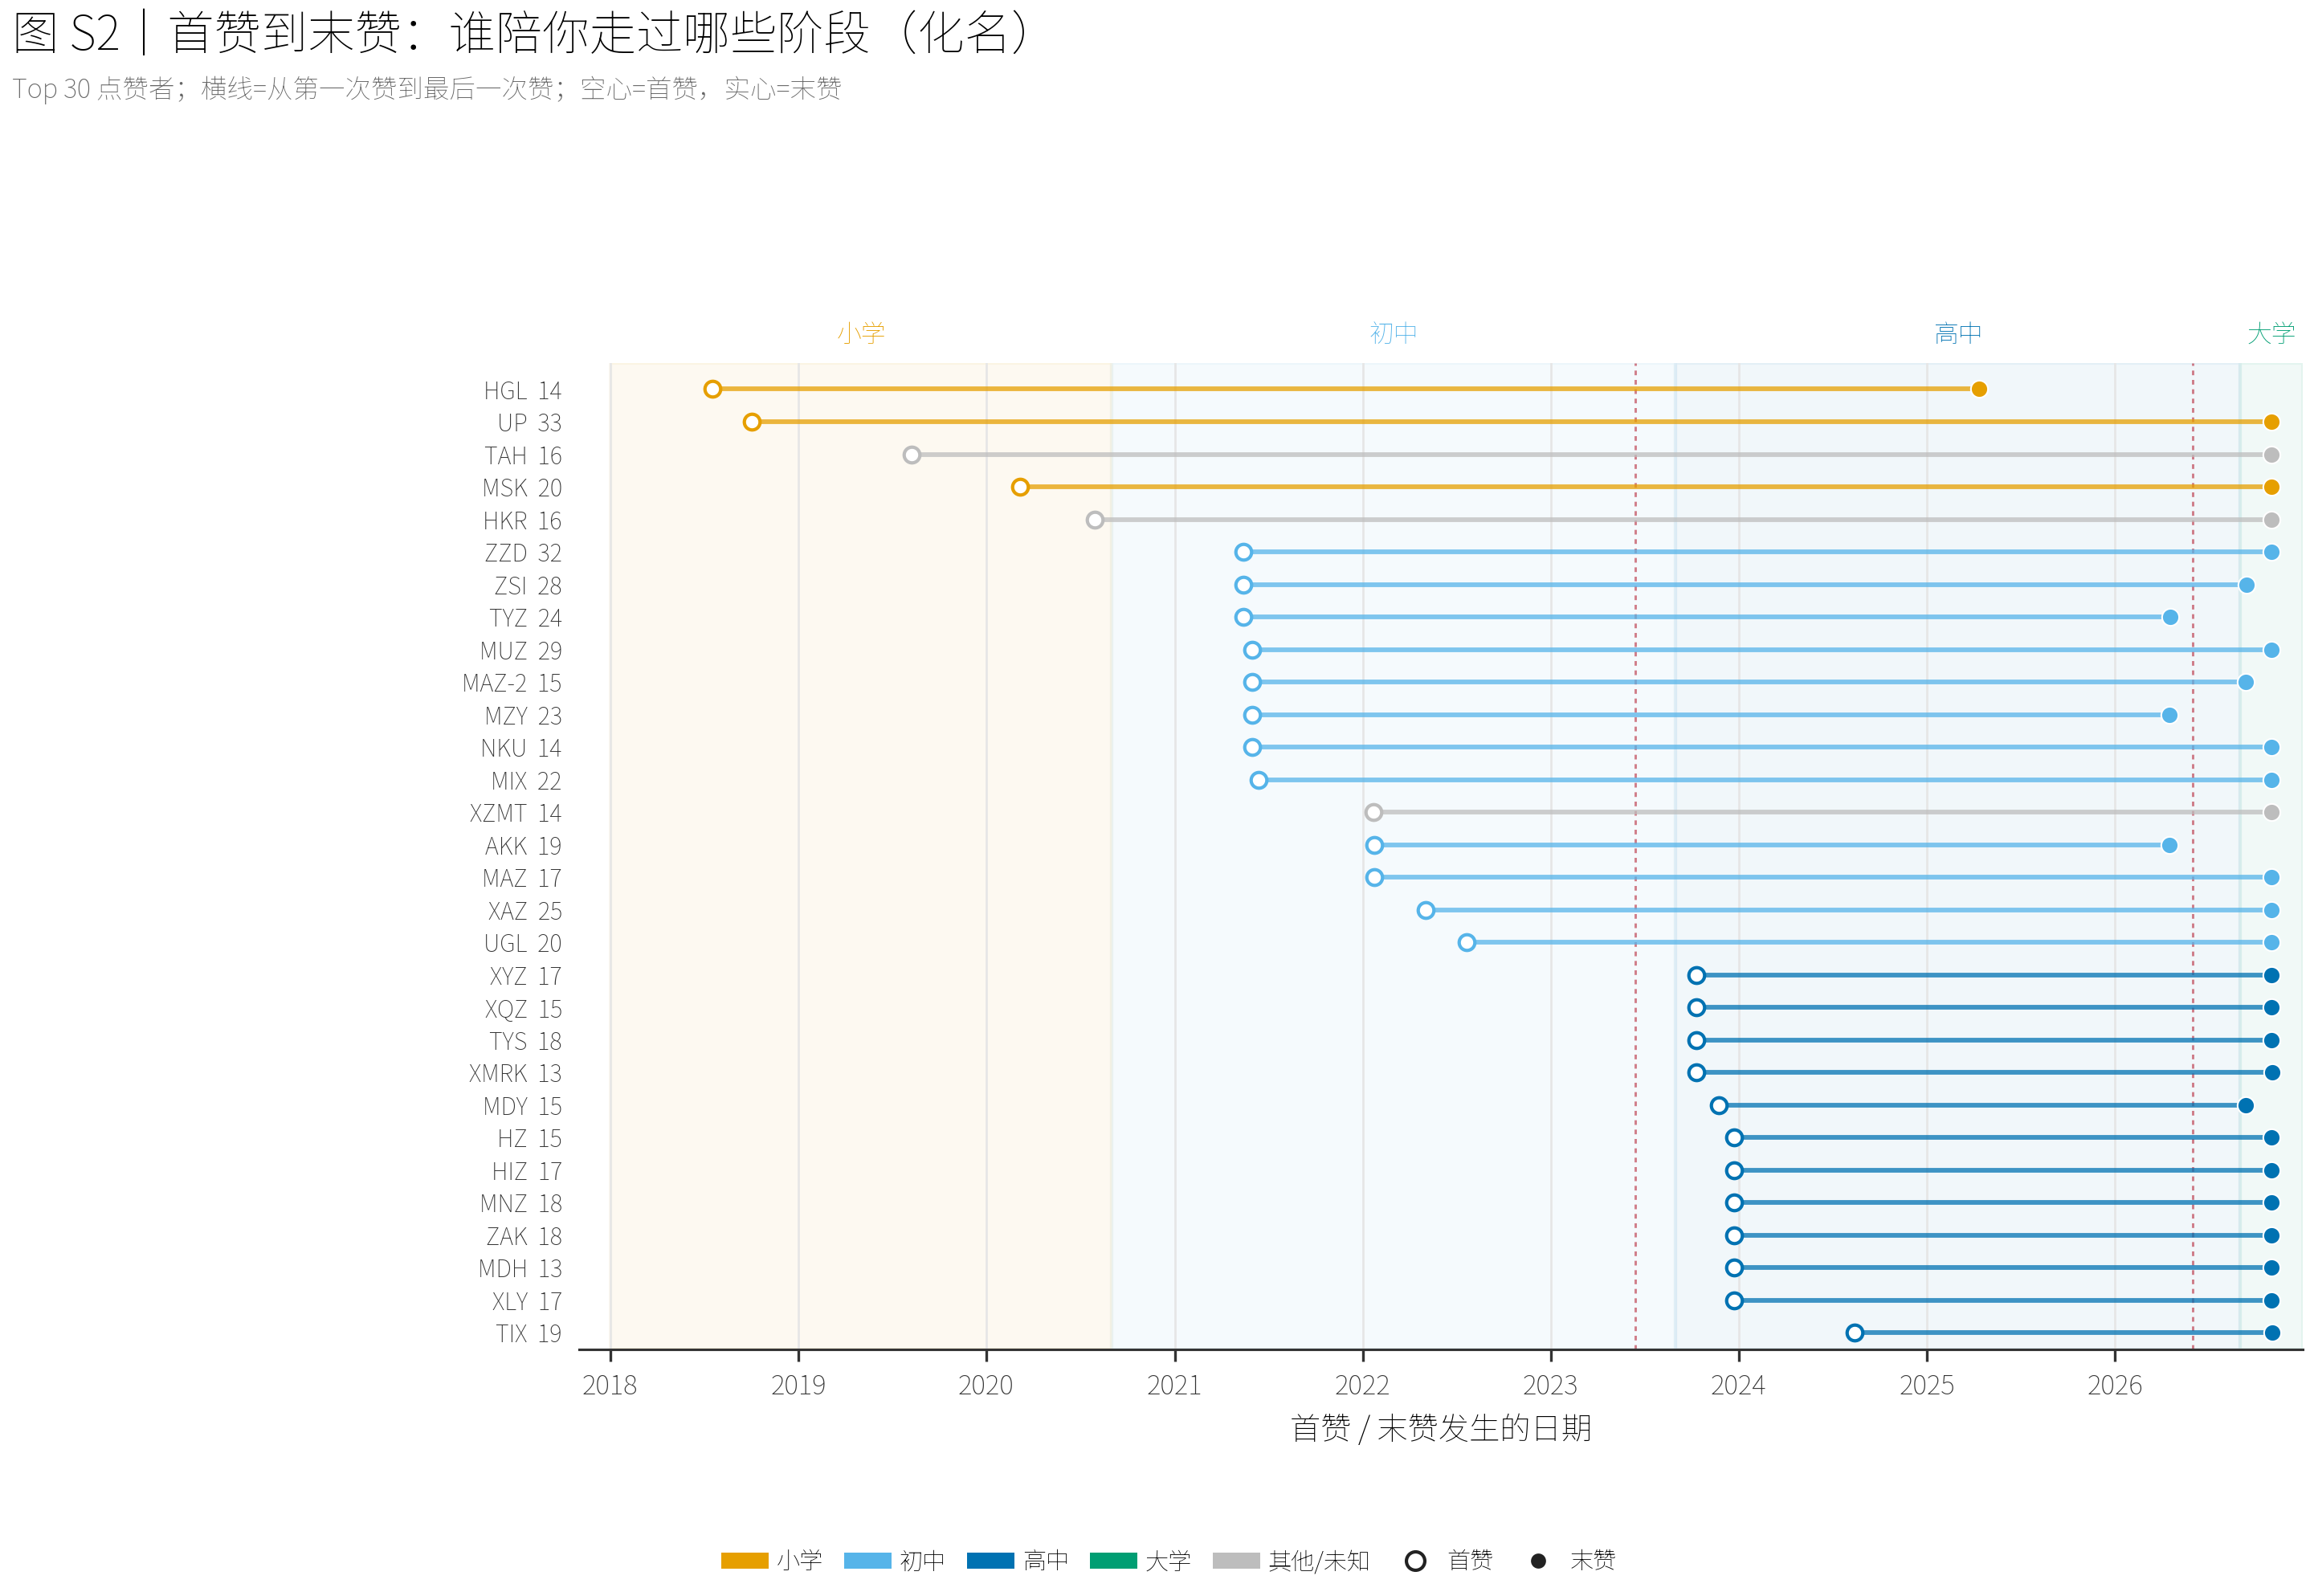
\includegraphics{assets/papers/moments-likes-analysis/figS2_lifelines_anon.png}}
\caption{图 S2：首赞到末赞的生命线。点赞次数最多的 30 位；空心=首赞，实心=末赞；颜色=最早关系阶段。}
\end{figure}

\begin{figure}
\centering
\href{assets/papers/moments-likes-analysis/figS3_stage_flow.png}{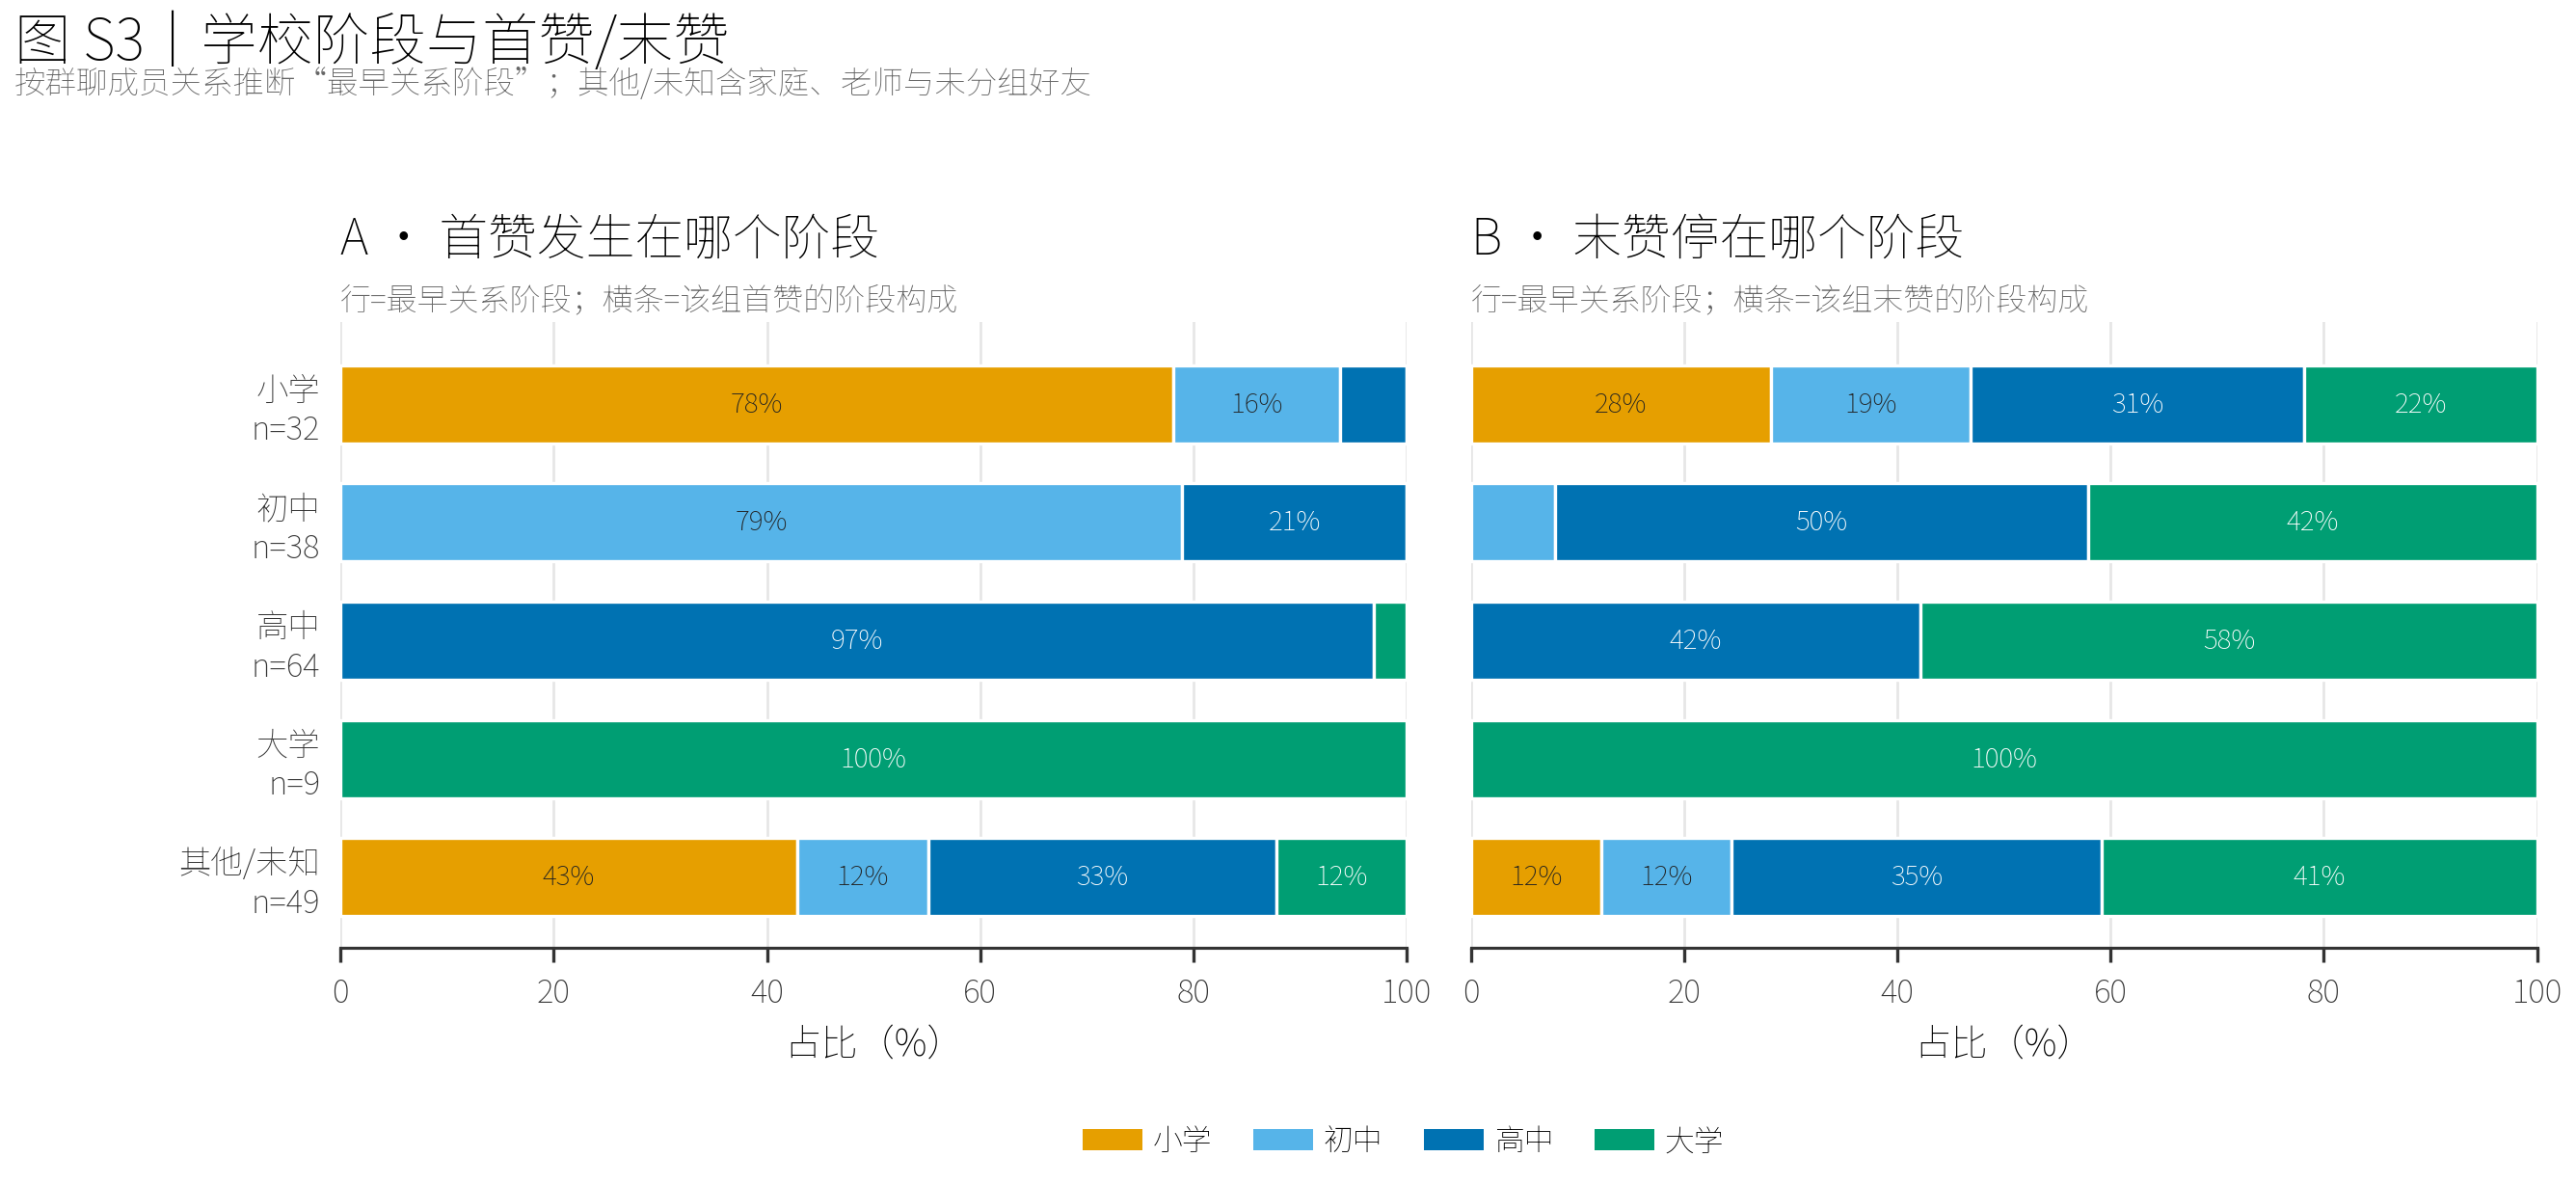
\includegraphics{assets/papers/moments-likes-analysis/figS3_stage_flow.png}}
\caption{图 S3：学校阶段与首赞/末赞构成。A：首赞阶段构成；B：末赞阶段构成；行=最早关系阶段。}
\end{figure}

\subsection{3.3 中考与高考}
2023 中考年：考前（1--6 月）0 条；考后（7--12 月）4 条，145 赞，均值 36.2，评论 27。2026 高考年：考前 1 条（4 月 16 日生日帖，69 赞、28 评论）；考后 5 条，227 赞，均值 45.4，评论 38。两年 6 月均为 0 条，考试月本身完全静默。

纵向看，2022 年 9 条，均值 27.0，评论 53；2023 年 4 条，均值 36.2，评论 27；2025 年 6 条，均值 43.7，评论 19；2026 年 6 条，均值 49.3，评论 66。2026 年的评论量明显上升；这既可能反映讨论意愿增强，也可能与高考后受众结构变化有关。

受众结构亦发生变化。2023 年考后帖的点赞者中，高中 47.6\%、初中 37.9\%、小学 9.0\%、其他 5.5\%；2026 年考后帖中，高中 44.5\%、初中 20.7\%、其他 20.7\%、大学 9.3\%、小学 4.8\%。初中占比减半，大学与其他新面孔补入。

\begin{table}[H]
\centering
\caption{表 5：中考/高考前后的发帖与互动。6 月为考试月。}
\footnotesize
\begin{tabular}{@{}l r r r r@{}}
\toprule
窗口 & n & 总赞 & 均值 & 评论 \\
\midrule
2023 考前（1–6 月） & 0 & 0 & — & 0 \\
2023 考后（7–12 月） & 4 & 145 & 36.2 & 27 \\
2026 考前（1–6 月） & 1 & 69 & 69.0 & 28 \\
2026 考后（7–12 月） & 5 & 227 & 45.4 & 38 \\
2022 全年 & 9 & 243 & 27.0 & 53 \\
2025 全年 & 6 & 262 & 43.7 & 19 \\
\bottomrule
\end{tabular}
\end{table}

\begin{figure}
\centering
\href{assets/papers/moments-likes-analysis/figS4_exams.png}{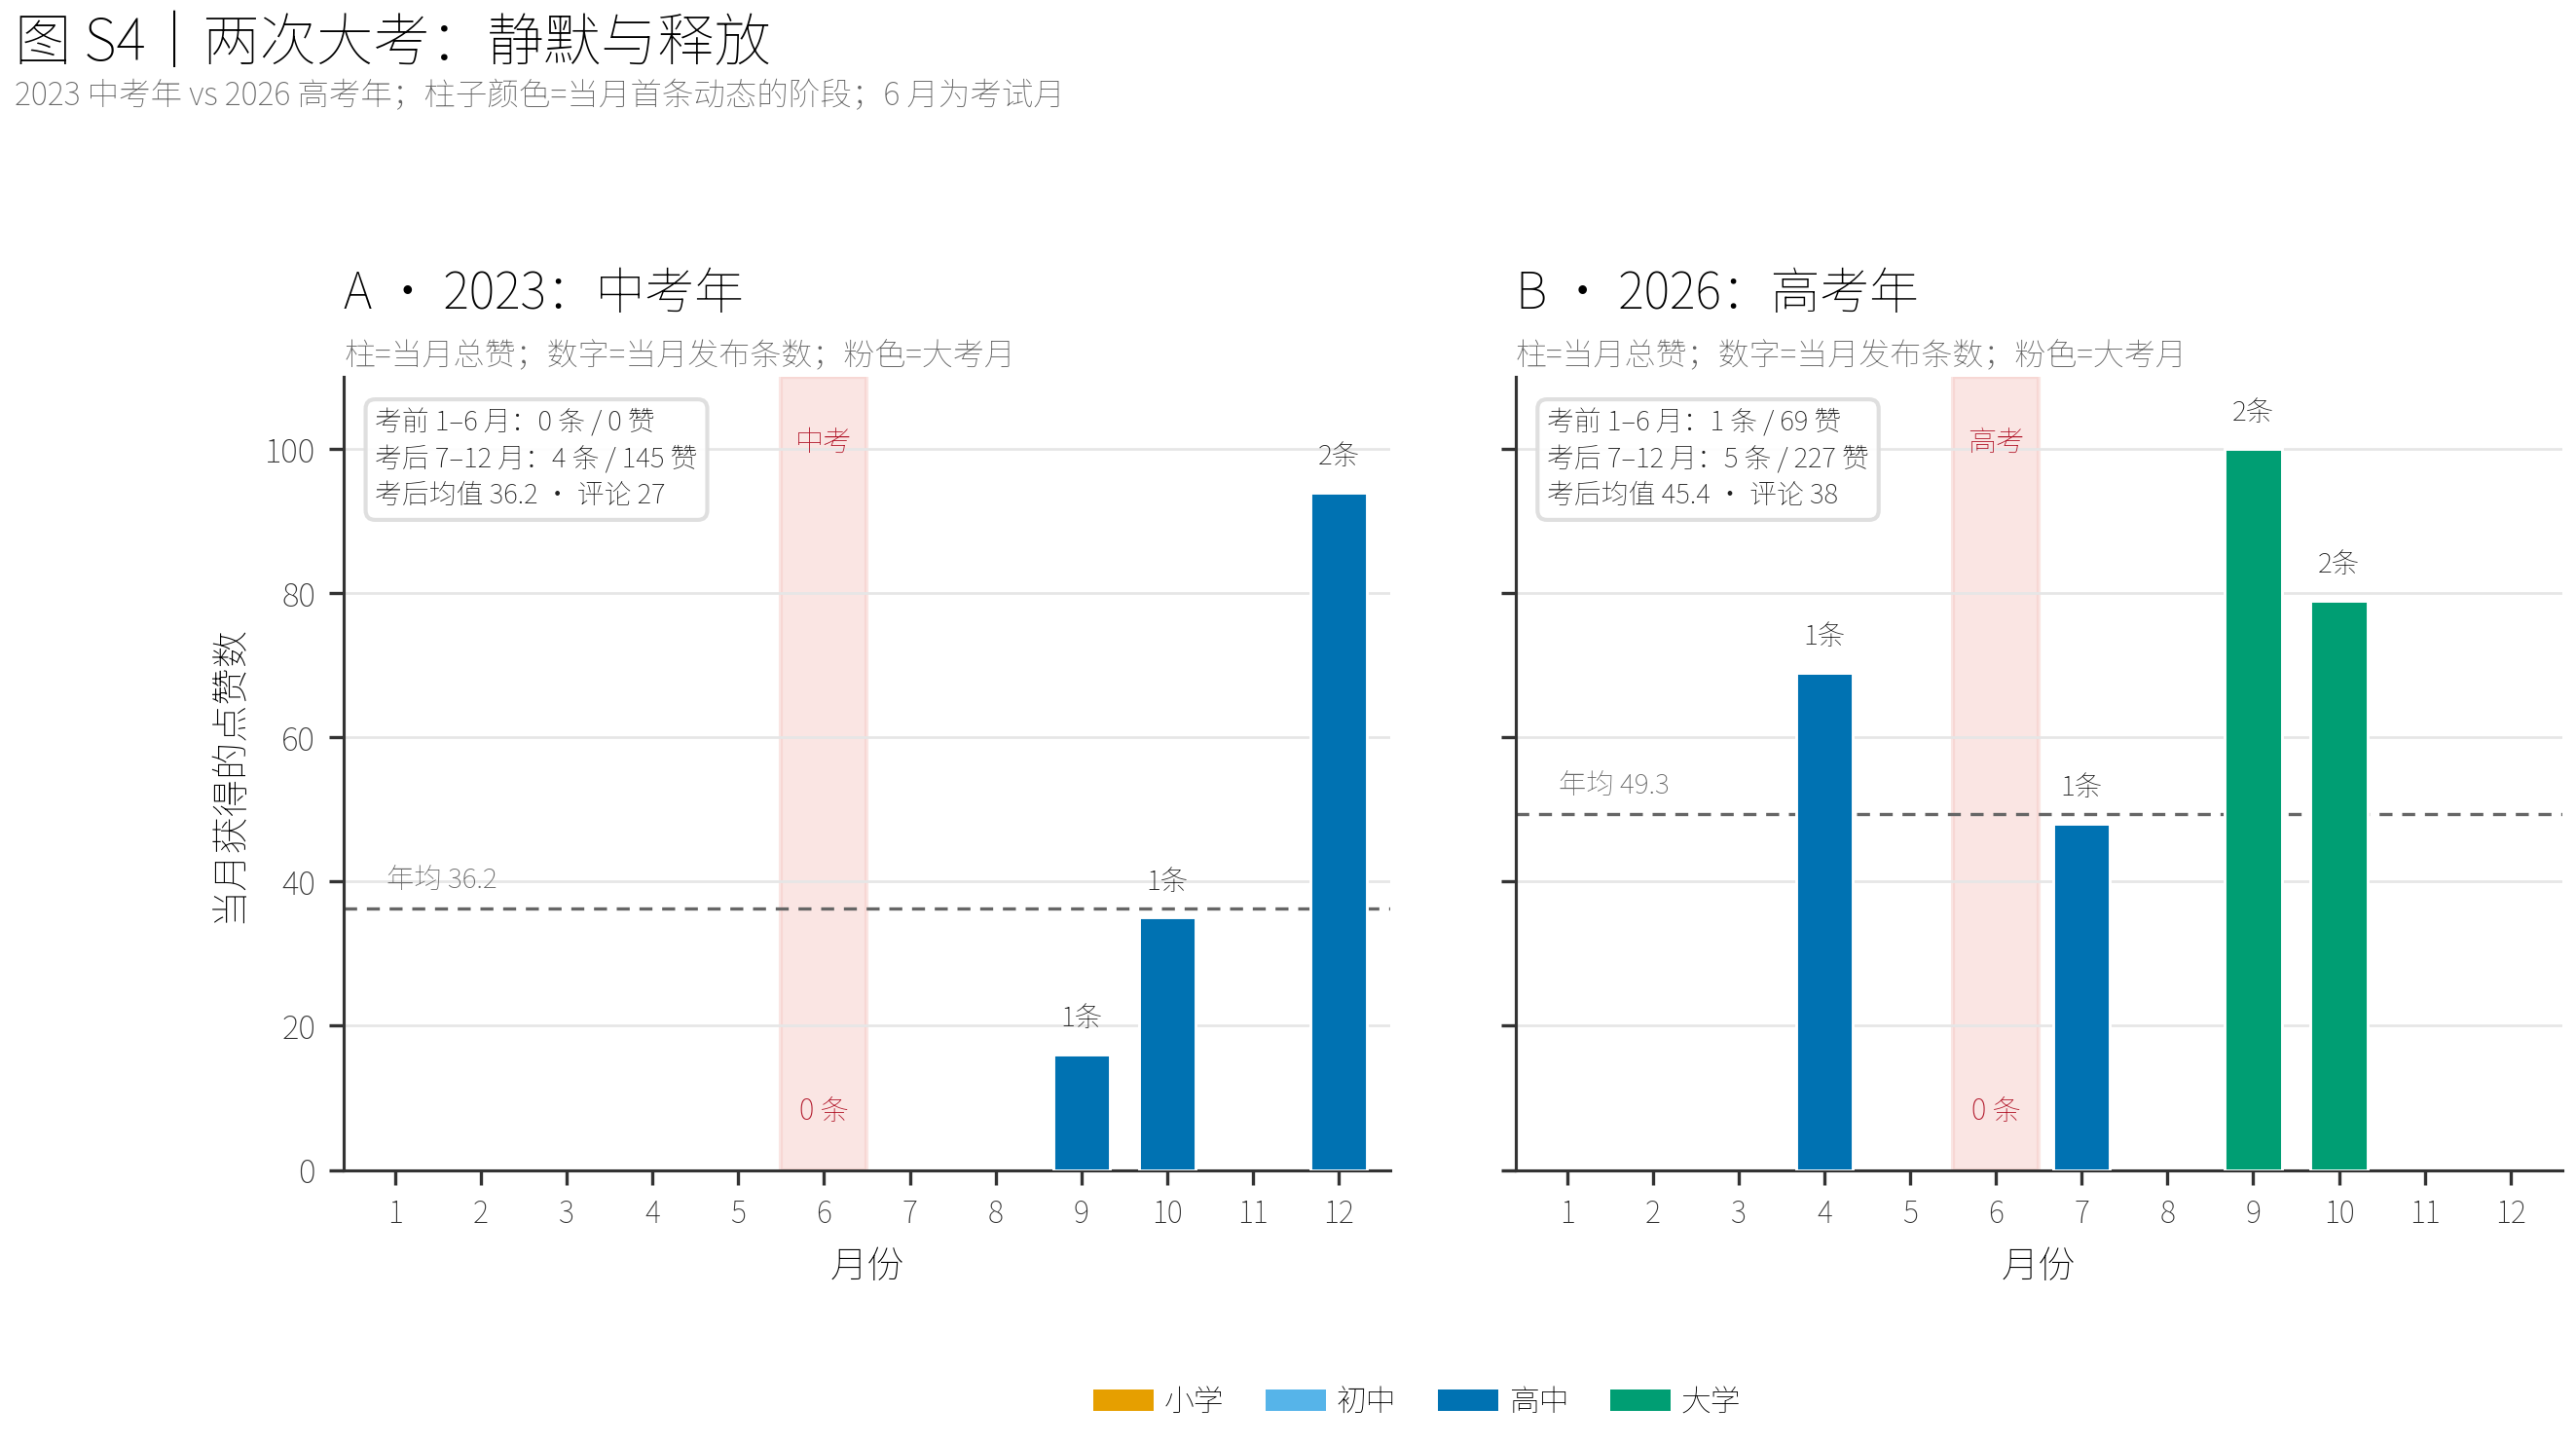
\includegraphics{assets/papers/moments-likes-analysis/figS4_exams.png}}
\caption{图 S4：两次大考：2023 中考年与 2026 高考年。柱=当月总赞；数字=当月发布条数；粉色=6 月考试月。}
\end{figure}

\section{4 讨论}
近三年的点赞量稳定在较高水平，但并非逐年上升：2024 年回落，2025--2026 年恢复。单条动态的点赞高度前置，近半数在 1 小时内到达，九成以上在 24 小时内完成。这一分布意味着，发布后的第一天是点赞形成的主要窗口；晚发主要让赞来得更快，而不改变最终规模。

内容类型之间的均值差异在统计上不显著，且样本量小。长文/月报的平均点赞最高，但仅 2 条；技术/项目的平均点赞最低，却有较高的评论/赞比。将点赞与评论合并看，内容类型更像“认可型”与“讨论型”的差异，而不是简单的“更受欢迎”与“更不受欢迎”。

核心点赞圈规模小、持续性强。前 8 位点赞者覆盖 85\%--90\% 的动态，前 10\% 点赞者贡献约三成点赞。核心成员以初中、高中阶段的关系为主，但这属于相关性描述；样本未包含关系强度、互动频率等变量，不能据此判断因果机制。

全历史补充分析显示，八年点赞数的线性上升（+5.40 赞/年）与受众规模变化一致；学校阶段队列呈现“小学起点、初中桥梁、高中与大学当前来源”的结构。两次大考前后均出现 6 月静默、考后恢复的模式；2026 年的评论量更高、大学与其他受众占比更大。上述补充结果用于提供纵向背景，不改变近三年主样本的结论。

\section{5 局限}
\begin{enumerate}[leftmargin=1.3em,itemsep=1pt,topsep=2pt]
\item 主样本仅 20 条动态，类别样本量为 2--6 条，置信区间较宽；所有 $p$ 值未做多重比较校正。
\item 数据来自单账号、单机缓存，可能遗漏未被客户端缓存的早期动态；近期帖子的点赞数仍可能继续增长。
\item 缺少曝光量、阅读量与好友规模等分母，无法区分“内容效应”与“到达效应”。
\item 内容类型为人工单编码；跨主题动态按主要篇幅归类，换一种编码规则可能改变边界。
\item 学校阶段由群聊成员关系推断，143/192 位点赞者可归类；一人可属于多个阶段，本文取最早阶段，可能存在误分类。
\item 已删除联系人仅保留本地可见记录；若删除时连点赞记录一并清除，本文无法恢复。
\item 观察性数据不能支持因果推断；时间、内容、受众与平台机制相互交织。
\end{enumerate}

\clearpage

\section*{附录 A：主样本 20 条动态的逐条指标}

\noindent\textbf{表 A1.} 主样本 20 条动态的点赞、评论、首小时点赞、半衰期与形式。赞/评论均不含本人；评论不含本人回复；半衰期单位为小时。
\vspace{2pt}

\footnotesize
\begin{longtable}{@{}r l l p{2.1cm} r r r r p{2.5cm}@{}}
\toprule
\# & 日期 & 阶段 & 类型 & 赞 & 评论 & 首小时 & 半衰期 & 形式 \\
\midrule

27 & 2023-12-22 & 高中 & 技术 / 项目 & 38 & 5 & 23 & 0.9 & 96字·无图 \\
28 & 2023-12-31 & 高中 & 长文 / 月报 & 56 & 7 & 29 & 0.9 & 1524字·3图 \\
30 & 2024-03-10 & 高中 & 旅行 / 自然 & 36 & 3 & 15 & 1.4 & 39字·3图 \\
31 & 2024-08-13 & 高中 & 旅行 / 自然 & 46 & 2 & 23 & 0.9 & 24字·9图 \\
32 & 2024-08-17 & 高中 & 校园 / 成长 & 27 & 2 & 9 & 2.9 & 123字·4图 \\
33 & 2024-08-26 & 高中 & 校园 / 成长 & 34 & 5 & 18 & 0.7 & 209字·9图 \\
34 & 2024-09-02 & 高中 & 旅行 / 自然 & 31 & 0 & 4 & 10.5 & 9字·9图 \\
35 & 2024-09-09 & 高中 & 旅行 / 自然 & 34 & 1 & 5 & 9.6 & 137字·9图 \\
36 & 2025-02-04 & 高中 & 校园 / 成长 & 24 & 0 & 7 & 2.7 & 9字·3图 \\
37 & 2025-04-09 & 高中 & 技术 / 项目 & 48 & 7 & 20 & 1.3 & 133字·9图·链接 \\
38 & 2025-04-11 & 高中 & 城市 / 影像 & 37 & 0 & 16 & 1.1 & 60字·9图 \\
39 & 2025-05-14 & 高中 & 校园 / 成长 & 47 & 1 & 22 & 1.3 & 70字·1图 \\
40 & 2025-05-19 & 高中 & 校园 / 成长 & 43 & 8 & 20 & 1.7 & 0字·1图 \\
41 & 2025-06-13 & 高中 & 旅行 / 自然 & 63 & 3 & 30 & 1.2 & 90字·6图 \\
42 & 2026-04-16 & 高中 & 校园 / 成长 & 69 & 28 & 27 & 4.7 & 77字·4图 \\
43 & 2026-07-23 & 高中 & 城市 / 影像 & 48 & 8 & 23 & 1.0 & 11字·9图 \\
44 & 2026-09-11 & 大学 & 城市 / 影像 & 61 & 8 & 41 & 0.5 & 74字·9图 \\
45 & 2026-09-26 & 大学 & 技术 / 项目 & 39 & 7 & 23 & 0.9 & 684字·无图·链接 \\
46 & 2026-10-11 & 大学 & 技术 / 项目 & 18 & 8 & 10 & 0.6 & 120字·无图·链接 \\
47 & 2026-10-31 & 大学 & 长文 / 月报 & 61 & 7 & 36 & 0.6 & 1395字·6图·链接 \\
\bottomrule
\end{longtable}
\normalsize

\vspace{0.5em}
\noindent\footnotesize 注：\#29 为 2023-12-31 16:46 的重复空帖，已剔除；4 次自赞已从对应帖子中剔除。形式列中的“字”为正文 Unicode 字符数，“图”为图片数，“链接”表示正文含 http(s) URL。

\section*{附录 B：全历史点赞次数 Top 15 的首赞与末赞}

\noindent\textbf{表 B1.} 全历史点赞次数最多的 15 位及其首赞/末赞。首/末赞按动作时间排序；帖子日期可能早于动作时间。关系=最早阶段。
\vspace{2pt}

\footnotesize
\begin{tabular}{@{}r p{2.0cm} r p{1.9cm} p{1.0cm} p{1.9cm} p{1.0cm} p{1.4cm}@{}}
\toprule
\# & 姓名 & 总赞 & 首赞 & 阶段 & 末赞 & 阶段 & 关系 \\
\midrule
1 & UP & 33 & \#2\newline 2018-06 & 小学 & \#47\newline 2026-10 & 大学 & 小学 \\
2 & ZZD & 32 & \#13\newline 2021-05 & 初中 & \#47\newline 2026-10 & 大学 & 初中 \\
3 & MUZ & 29 & \#14\newline 2021-05 & 初中 & \#47\newline 2026-10 & 大学 & 初中 \\
4 & ZSI & 28 & \#13\newline 2021-05 & 初中 & \#44\newline 2026-09 & 大学 & 初中 \\
5 & XAZ & 25 & \#20\newline 2022-05 & 初中 & \#47\newline 2026-10 & 大学 & 初中 \\
6 & TYZ & 24 & \#13\newline 2021-05 & 初中 & \#42\newline 2026-04 & 高中 & 初中 \\
7 & MZY & 23 & \#14\newline 2021-05 & 初中 & \#42\newline 2026-04 & 高中 & 初中 \\
8 & MIX & 22 & \#15\newline 2021-06 & 初中 & \#47\newline 2026-10 & 大学 & 初中 \\
9 & MSK & 20 & \#10\newline 2020-03 & 小学 & \#47\newline 2026-10 & 大学 & 小学 \\
10 & UGL & 20 & \#21\newline 2022-07 & 初中 & \#47\newline 2026-10 & 大学 & 初中 \\
11 & TIX & 19 & \#31\newline 2024-08 & 高中 & \#47\newline 2026-10 & 大学 & 高中 \\
12 & AKK & 19 & \#16\newline 2022-01 & 初中 & \#42\newline 2026-04 & 高中 & 初中 \\
13 & TYS & 18 & \#26\newline 2023-10 & 高中 & \#47\newline 2026-10 & 大学 & 高中 \\
14 & ZAK & 18 & \#27\newline 2023-12 & 高中 & \#47\newline 2026-10 & 大学 & 高中 \\
15 & MNZ & 18 & \#27\newline 2023-12 & 高中 & \#47\newline 2026-10 & 大学 & 高中 \\
\bottomrule
\end{tabular}
\normalsize

\section*{附录 C：编码规则}

\begin{itemize}[leftmargin=1.3em,itemsep=2pt,topsep=2pt]
\item \textbf{长文/月报}：年度总结、站点月报、以完整叙事为主的长文。
\item \textbf{城市/影像}：城市摄影、骑行、季节影像，文字多为短句或图注。
\item \textbf{技术/项目}：软件发布、项目/站点更新、开发月报。
\item \textbf{旅行/自然}：登山、旅行、自然风景。
\item \textbf{校园/成长}：课程实验、校园建筑、演出/活动、考试与成长反思。
\end{itemize}
编码为人工单编码，优先看正文主题；图文并茂时以文字主题为准。跨主题动态按主要篇幅归类。学校阶段由群聊名称中的小学、初中、高中、大学相关关键词推断；多阶段时取最早阶段。
